\documentclass{foi}

\usepackage[document]{ragged2e}

\vrstaRada{\zavrsni} % \diplomski
\title{Prilagodljiv sustav za smanjenje svjetlosnog zasljepljivanja vozača}

\author{Stjepan Petrović}
\spolStudenta{\musko} % \zensko ili \musko
\mentor{Boris Tomaš}
\spolMentora{\musko} % \zensko ili \musko
\godina{2023}
\mjesec{rujan}
\date{2023}
\status{redoviti}
\indeks{0016150314}
\smjer{Informacijski i poslovni sustavi} % (ili Poslovni sustavi, Ekonomika poduzetništva, Primjena informacijske tehnologije u poslovanju, Informacijsko i programsko inženjerstvo, Baze podataka i baze znanja, Organizacija poslovnih sustava, Informatika u obrazovanju)
\titulaProfesora{Doc. dr. sc.}

\sazetak{Tema rada je izrada prilagodljivog sustava za smanjenje svjetlosnog zasljepljivanja vozača što predstavlja fizički koncept koji čini LCD matrica, dvije web kamere i laptop kao procesna jedinica. Izazov je bio spojiti četiri komponente (komponenta za pozicioniranje očiju vozača, komponenta za pozicioniranje zasljepljujućeg svjetla, komponenta za zaštitu od zasljepljujućeg svjetla i komponenta procesne jedinice zajedno sa ostalim hardverom), od kojih svaka ima svoju važnost i način pristupa, u jedan funkcionalan sustav čiji je koncept realiziran u ovome radu i koji odgovara na pitanje: kako preko kamera prepoznati izvor zasljepljujućeg svjetla i zaštiti oči vozača na način da se preko LCD matrice spriječi prolazak zasljepljujućeg svjetla do očiju vozača. Kako bi se izradio odgovarajući sustav korištena je biblioteka OpenCV (engl. \emph{Open Source Computer Vision Library}) koja je kao projekt pokrenuta od strane Intel korporacije, a pruža softver za strojno učenje i računalni vid u realnom vremenu i korišten je programski jezik Python. Programski kod i \LaTeX \space dokumentacija je verzionizirana na GitHub repozitoriju, kojem se može pristupiti preko poveznice: \url{https://github.com/StjepanPetrovic/Prilagodljiv-sustav-za-smanjenje-svjetlosnog-zasljepljivanja-vozaca}.}

\kljucneRijeci{računalni vid; OpenCV; vozilo; zasljepljivanje; LCD; Python;}

\begin{document}

\justifying

\counterwithout{lstlisting}{chapter}

\captionsetup[lstlisting]{font={small, sf},labelfont={sf, small}}

\maketitle

\tableofcontents

\pagestyle{plain}
\chapter{Uvod}

Ovim završnim radom obrađeni su teorijski koncepti na kojima se temelji rad, istražena je literatura, opisan je tijek izrade i konačan rezultat izrade \textbf{prilagodljivog sustava za smanjenje svjetlosnog zasljepljivanja vozača} te je provedeno testiranje sustava.

U nastavku rada za izraz „prilagodljiv sustav za smanjenje svjetlosnog zasljepljivanja vozača koristit će se skraćena inačica „\textbf{sustav protiv zasljepljivanja}“.

\section{Definicija problema}

 Bilo je potrebno napraviti sustav koji u realnom vremenu prepoznaje izvor zasljepljujućeg svjetla te reagira na način da polarizira određeni dio reaktivne komponente (LCD matrice) koja bi se nalazila na vjetrobranskom staklu vozila te na taj način smanji jačinu zasljepljujućeg svjetla ispred vozača u vozilu.

 Na slici \ref{fig:prikaz_sustava_1} može se vidjeti da takav sustav treba imati ulazne uređaje pomoću kojih će vidjeti što se događa u okolini vozača. Za ulazne uređaje su uzete dvije web kamere čiji je sadržaj onoga što vide predstavljen kao narančasti i zeleni okvir na slici \ref{fig:prikaz_sustava_1}, a taj sadržaj će obrađivati istrenirani modeli za računalni vid iz biblioteke OpenCV te će tako procesna jedinica znati gdje se nalaze oči vozača i izvor svjetla koji su predstavljeni kao crveni krugovi odnosno baze valjka na narančastom i zelenom okviru na slici \ref{fig:prikaz_sustava_1}. Kada procesna jedinica to zna, potrebno je pomoću algoritma izračunati koji točno dio LCD matrice treba polarizirati/zatamniti, a taj dio koji treba polarizirati je prikazan na slici \ref{fig:prikaz_sustava_1} kao crveni krug na crnom okviru odnosno intersekcija žutog plašta valjka, koji predstavlja svjetlost, sa crnim okvirom koji predstavlja reaktivnu komponentu (LCD matricu). Interaktivnom grafu sa slike \ref{fig:prikaz_sustava_1} može se pristupiti preko linka: \url{https://www.geogebra.org/m/hvzfyjfz}.


\begin{figure}[h!]
    \centering
    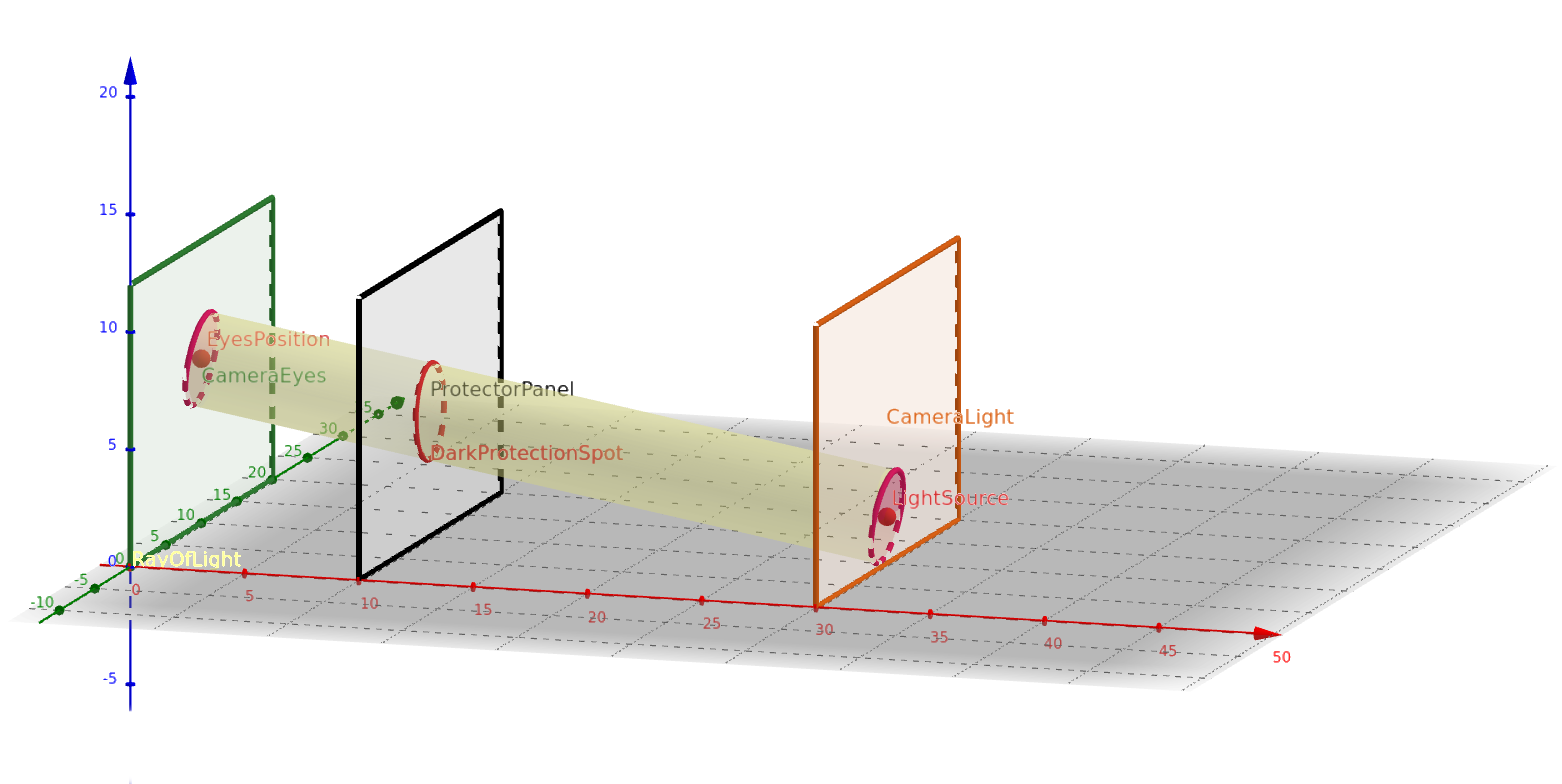
\includegraphics[width=0.75\textwidth]{slike/graf_uvod}
    \captionsetup{font={small}}
    \caption{Pojednostavljen prikaz sustava u trodimenzionalnom koordinatnom sustavu [autorski rad]}
    \label{fig:prikaz_sustava_1}
\end{figure}

Razlog zbog čega je uzeta LCD matrica kao reaktivna komponenta koja će sprječavati zasljepljujuće svjetlo da dođe do očiju vozača je taj što može biti prozirna i moguće je gledati kroz nju, zbog čega neće smetati na vjetrobranskom staklu prilikom vožnje, a lako ju je moguće napraviti neprozirnom na način da se zaslon polarizira odnosno da se pikseli postave na crnu boju.

\begin{flushleft}Sustav protiv zasljepljivanja se sastoji od četiri komponente koje su u radu obrađena:\end{flushleft}
\begin{itemize}[noitemsep]
    \item Procesna jedinica (laptop) i hardver (web kamere i LCD matrica),
    \item Komponenta za prepoznavanje i pozicioniranje izvora svjetla,
    \item Komponenta za prepoznavanje i pozicioniranje očiju vozača,
    \item Komponenta za polarizaciju LCD matrice kao reaktivne komponente.
\end{itemize}

Uz dodatna ulaganja i razvoj, ovaj fizički koncept može postati vrlo popularan i koristan proizvod svakom vozaču u vozilu jer će pružiti zaštitu u noćnoj vožnji od zasljepljujuće svjetlosti, koja usmjerena u oči vozača za vrlo kratak trenutak može ugroziti vozača. Najčešće su izvor te svjetlosti duga svjetla na vozilu vozača koji zbog neopreznosti ne isključi duga svjetla u trenutku kada dolazi ususret drugom vozilu čiji će vozač zbog toga biti svjetlosno zaslijepljen te na trenutak neće moći vidjeti kuda vozi što može loše utjecati na vozača. Zato je bilo potrebno napraviti sustav koji će:
\begin{itemize}[noitemsep]
    \item prepoznati i pozicionirati izvor svjetla te oči vozača koristeći kamere,
    \item kalibrirati komponente i uspješno ih povezati u jedan cjelovit funkcionalan sustav.
\end{itemize}

\section{Motivacija za rad}

Motivacija za odabir ove teme mi je bila misao da ću se okušati u stvaranju sustava protiv zasljepljivanja za kojeg i u modernoj automobilskoj industriji još ne postoji izrađeno rješenje koje je optimalno za korištenje u realnim uvjetima – zbog čega sam gore i rekao da bi uz daljnja ulaganja i razvoj,  fizički koncept koji je izrađen u svrhu ovog završnog rada mogao biti popularan. Postoji velik broj raspisanih patenata od strane najkonkurentnijih svjetskih proizvođača što ostavlja dojam da će skorija budućnost biti jako dinamična utrka za osvajanje tržišta proizvodom koji će, osim borbe sa svjetlosnim zasljepljenjem, donijeti i dodatne mogućnosti kao što je uvođenje proširene stvarnosti (engl. \emph{Augmented Reality - AR}) na vjetrobransko staklo.

Velik je broj nesreća prouzrokovan svjetlosnim zasljepljenjem vozača, a još veći je broj vozila koji se svakim danom povećava na prometnicama širom svijeta, stoga moderna automobilska industrija sve više pokušava proizvesti automobile koji će imati ugrađen takav sustav za zaštitu vozača – što donosi velik značaj ovoj temi te poticaj za daljnje istraživanje i razvoj proizvoda koji će spriječiti povećanje broja prometnih nesreća prouzrokovanih svjetlosnim zasljepljenjem vozača.

\section{Metode i tehnike rada}

U ovom poglavlju treba opisati koje će metode i tehnike biti korištene pri razradi teme, kako su provedene istraživačke aktivnosti, koji su programski alati ili aplikacije korišteni.

Programski kod i \LaTeX \space dokumentacija je verzionizirana na GitHub repozitoriju, kojem se može pristupiti preko poveznice: \href{https://github.com/StjepanPetrovic/Prilagodljiv-sustav-za-smanjenje-svjetlosnog-zasljepljivanja-vozaca}{https://github.com/StjepanPetrovic/Prilagodljiv-sustav-za-smanjenje-svjetlosnog-zasljepljivanja-vozaca}.

\chapter{Pregled literature}

\chapter{Izrada sustava}

U ovom poglavlju će biti opisana izrada prilagodljivog sustava za smanjenje svjetlosnog zasljepljivanja vozača. Ovo će poglavlje biti podijeljeno na četiri potpoglavlja od kojih će svaki opisivati određenu komponentu budući da se sustav sastoji od četiri komponente:
\begin{itemize}[noitemsep]
    \item procesna jedinica (laptop) i hardver (web kamere i LCD matrica),
    \item komponenta za prepoznavanje i pozicioniranje izvora svjetla,
    \item komponenta za prepoznavanje i pozicioniranje očiju vozača,
    \item komponenta za polarizaciju LCD matrice kao reaktivne komponente.
\end{itemize}

Programski kod koji se bude prikazivao u radu može se pronaći na GitHub repozitoriju preko poveznice: \href{https://github.com/StjepanPetrovic/Prilagodljiv-sustav-za-smanjenje-svjetlosnog-zasljepljivanja-vozaca}{https://github.com/StjepanPetrovic/Prilagodljiv-sustav-za-smanjenje-svjetlosnog-zasljepljivanja-vozaca}. Svi isječci programskog koda su uzeti iz jedne datoteke \href{https://github.com/StjepanPetrovic/Prilagodljiv-sustav-za-smanjenje-svjetlosnog-zasljepljivanja-vozaca/blob/main/development/main.py}{$main.py$} te će se u isječcima programskog koda moći vidjeti i redni brojevi linija koda koji se odnose na redne brojeve linija koda iz datoteke \href{https://github.com/StjepanPetrovic/Prilagodljiv-sustav-za-smanjenje-svjetlosnog-zasljepljivanja-vozaca/blob/main/development/main.py}{$main.py$}.

Ovim radom izrađen je koncept koji će objasniti i prikazati ideju za izradu ovakvog sustava, ali ovaj koncept nije spreman za upotrebu u stvarnoj okolini. Ono što nije ovim radom obrađeno je navedeno u nastavku, to su neke od glavnih značajki koje bi sustav trebao ispunjavati kako bi pronašao svrhu u stvarnoj okolini:
\begin{itemize}[noitemsep]
    \item korištenje mikroprocesora koji će biti zadužen samo za obavljanje funkcionalnosti sustava,
    \item korištenje posebno izrađene prozirne LCD matrice ili korištenje drugog medija kao reaktivne komponente koja bi poslužila svrsi,
    \item korištenje posebnog modela i senzora za otkrivanje jačine svjetlosti,
    \item korištenje posebno istreniranog modela ili senzora koji će moći izračunati udaljenost zasljepljujućeg svjetla i očiju od reaktivne komponente,
    \item korištenje algoritma koji će uzeti u obzir sve udaljenosti, nagib vjetrobranskog stakla i klasifikacije objekata od interesa kako bi što kvalitetnije izračunavao mjesto na kojemu treba zaustaviti svjetlost preko reaktivne komponente,
    \item spremnost na rad u noćnim uvjetima,
    \item velika količina testiranja sustava u raznovrsnoj i dinamičnoj okolini (posebno noćnoj okolini).
\end{itemize}

\pagebreak
\section{Komponenta procesne jedinice i hardver}

Ovo poglavlje opisuje komponentu procesne jedinice kao komponentu koja čini temelj i softverski povezuje ostale komponente, a također opisuje i kako je sustav hardverski povezan.

\subsection{Hardver}
U ovom radu komponentu procesne jedinice predstavlja laptop na kojem će se izvršavati programski kod i čiji će procesor obrađivati ulazne informacije koje šalju kamere, a kamere su obične web kamere od kojih je jedna ugrađena u laptop, a druga je eksterna i priključena je preko USB priključka u laptop. Jedna kamera je namjenjena za snimanje okoline ispred vozača, a druga kamera je namijenjena za snimanje samog vozača.

Ispred vozača bi se nalazila LCD matrica koja će smanjiti i sprječiti zasljepljujuću svjetlost da dođe do očiju vozača. LCD matrica, zajedno sa elektronikom, za ovaj rad je izvađena iz običnog monitora te povezana preko HDMI priključka u laptop i ponaša se kao drugi zaslon laptopa. Na slici \ref{fig:lcd_matrica_1} i \ref{fig:lcd_matrica_2} može se vidjeti kako izgleda LCD matrica zajedno sa elektronikom i priključcima kada je izvađena iz monitora. Kao što se može vidjeti, LCD matrica kada se izvadi iz monitora je tamna te je potrebno imati jak izvor svjetla kako bi se vidjelo kroz nju dok je samostalno izvan monitora. TODO - iz toga razloga planiram postaviti LED svjetla iznad i ispod LCD matrice kako bih poboljšao njezinu providnost.

\begin{figure}[h!]
    \centering
    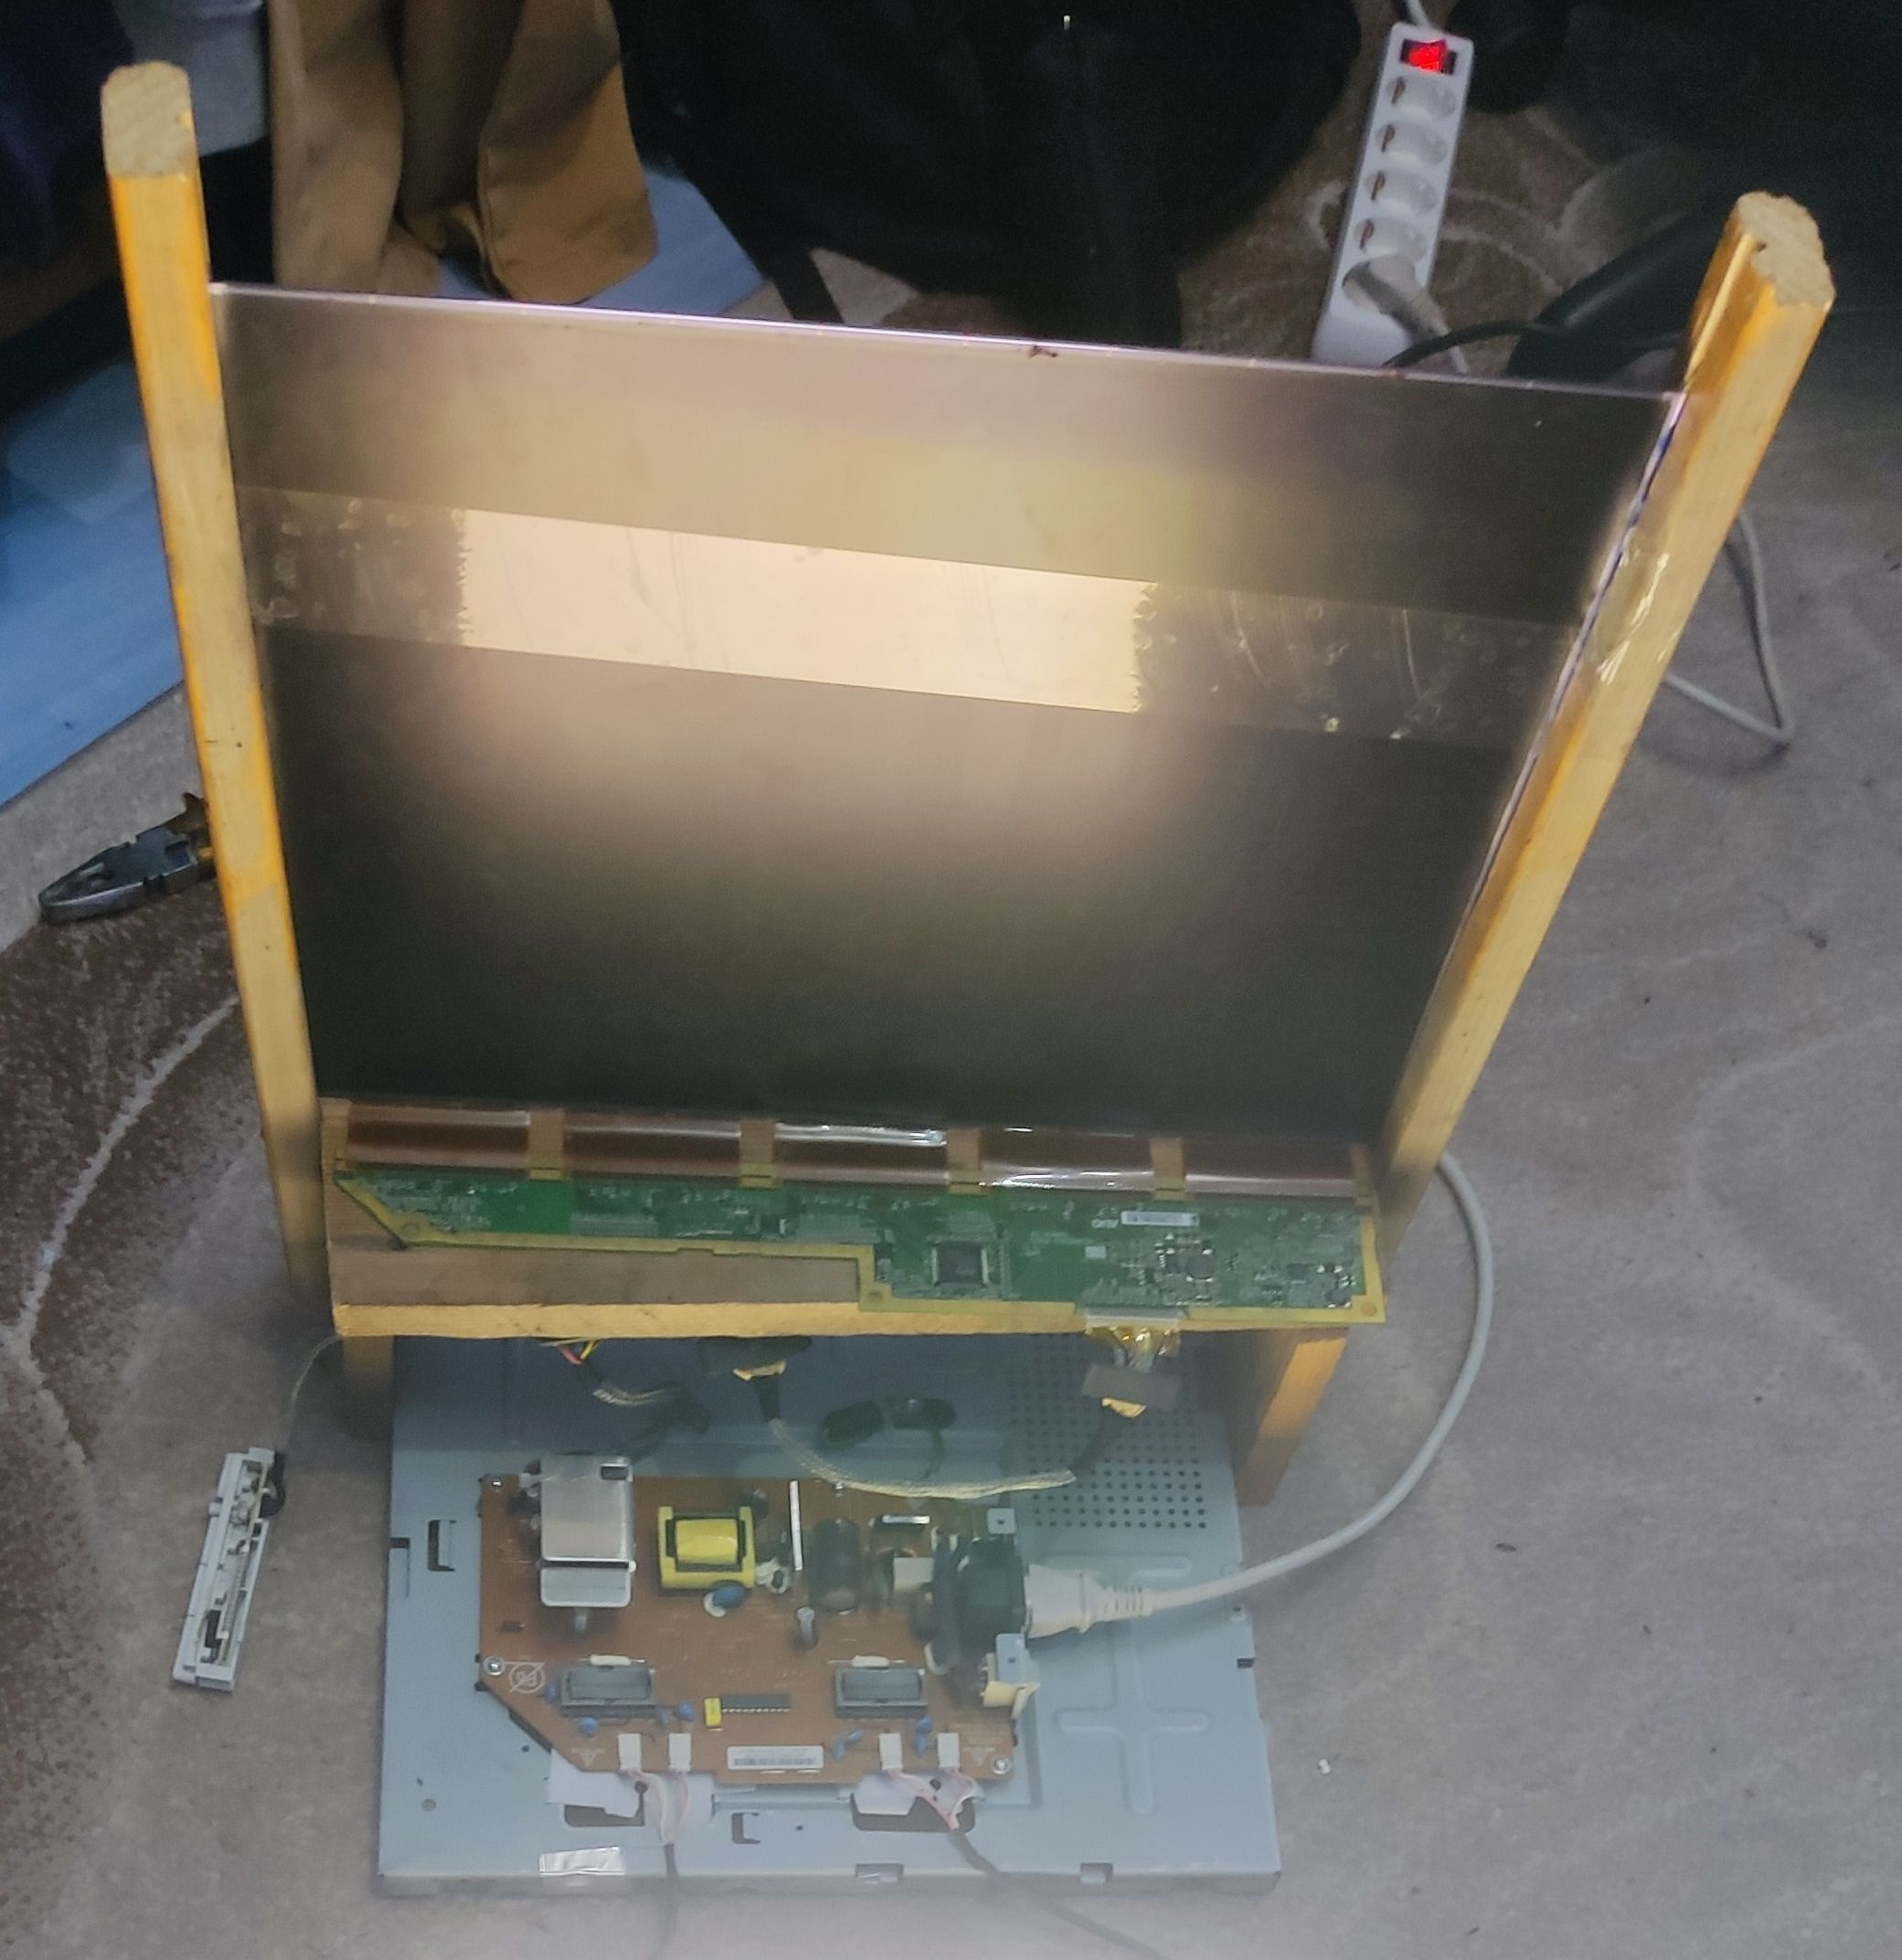
\includegraphics[width=0.5\textwidth]{slike/lcd_matrica_1}
    \captionsetup{font={small}}
    \caption{Prikaz LCD matrica s prednje strane kada je izvađena iz monitora [autorski rad]}
    \label{fig:lcd_matrica_1}
\end{figure}

\begin{figure}[h!]
    \centering
    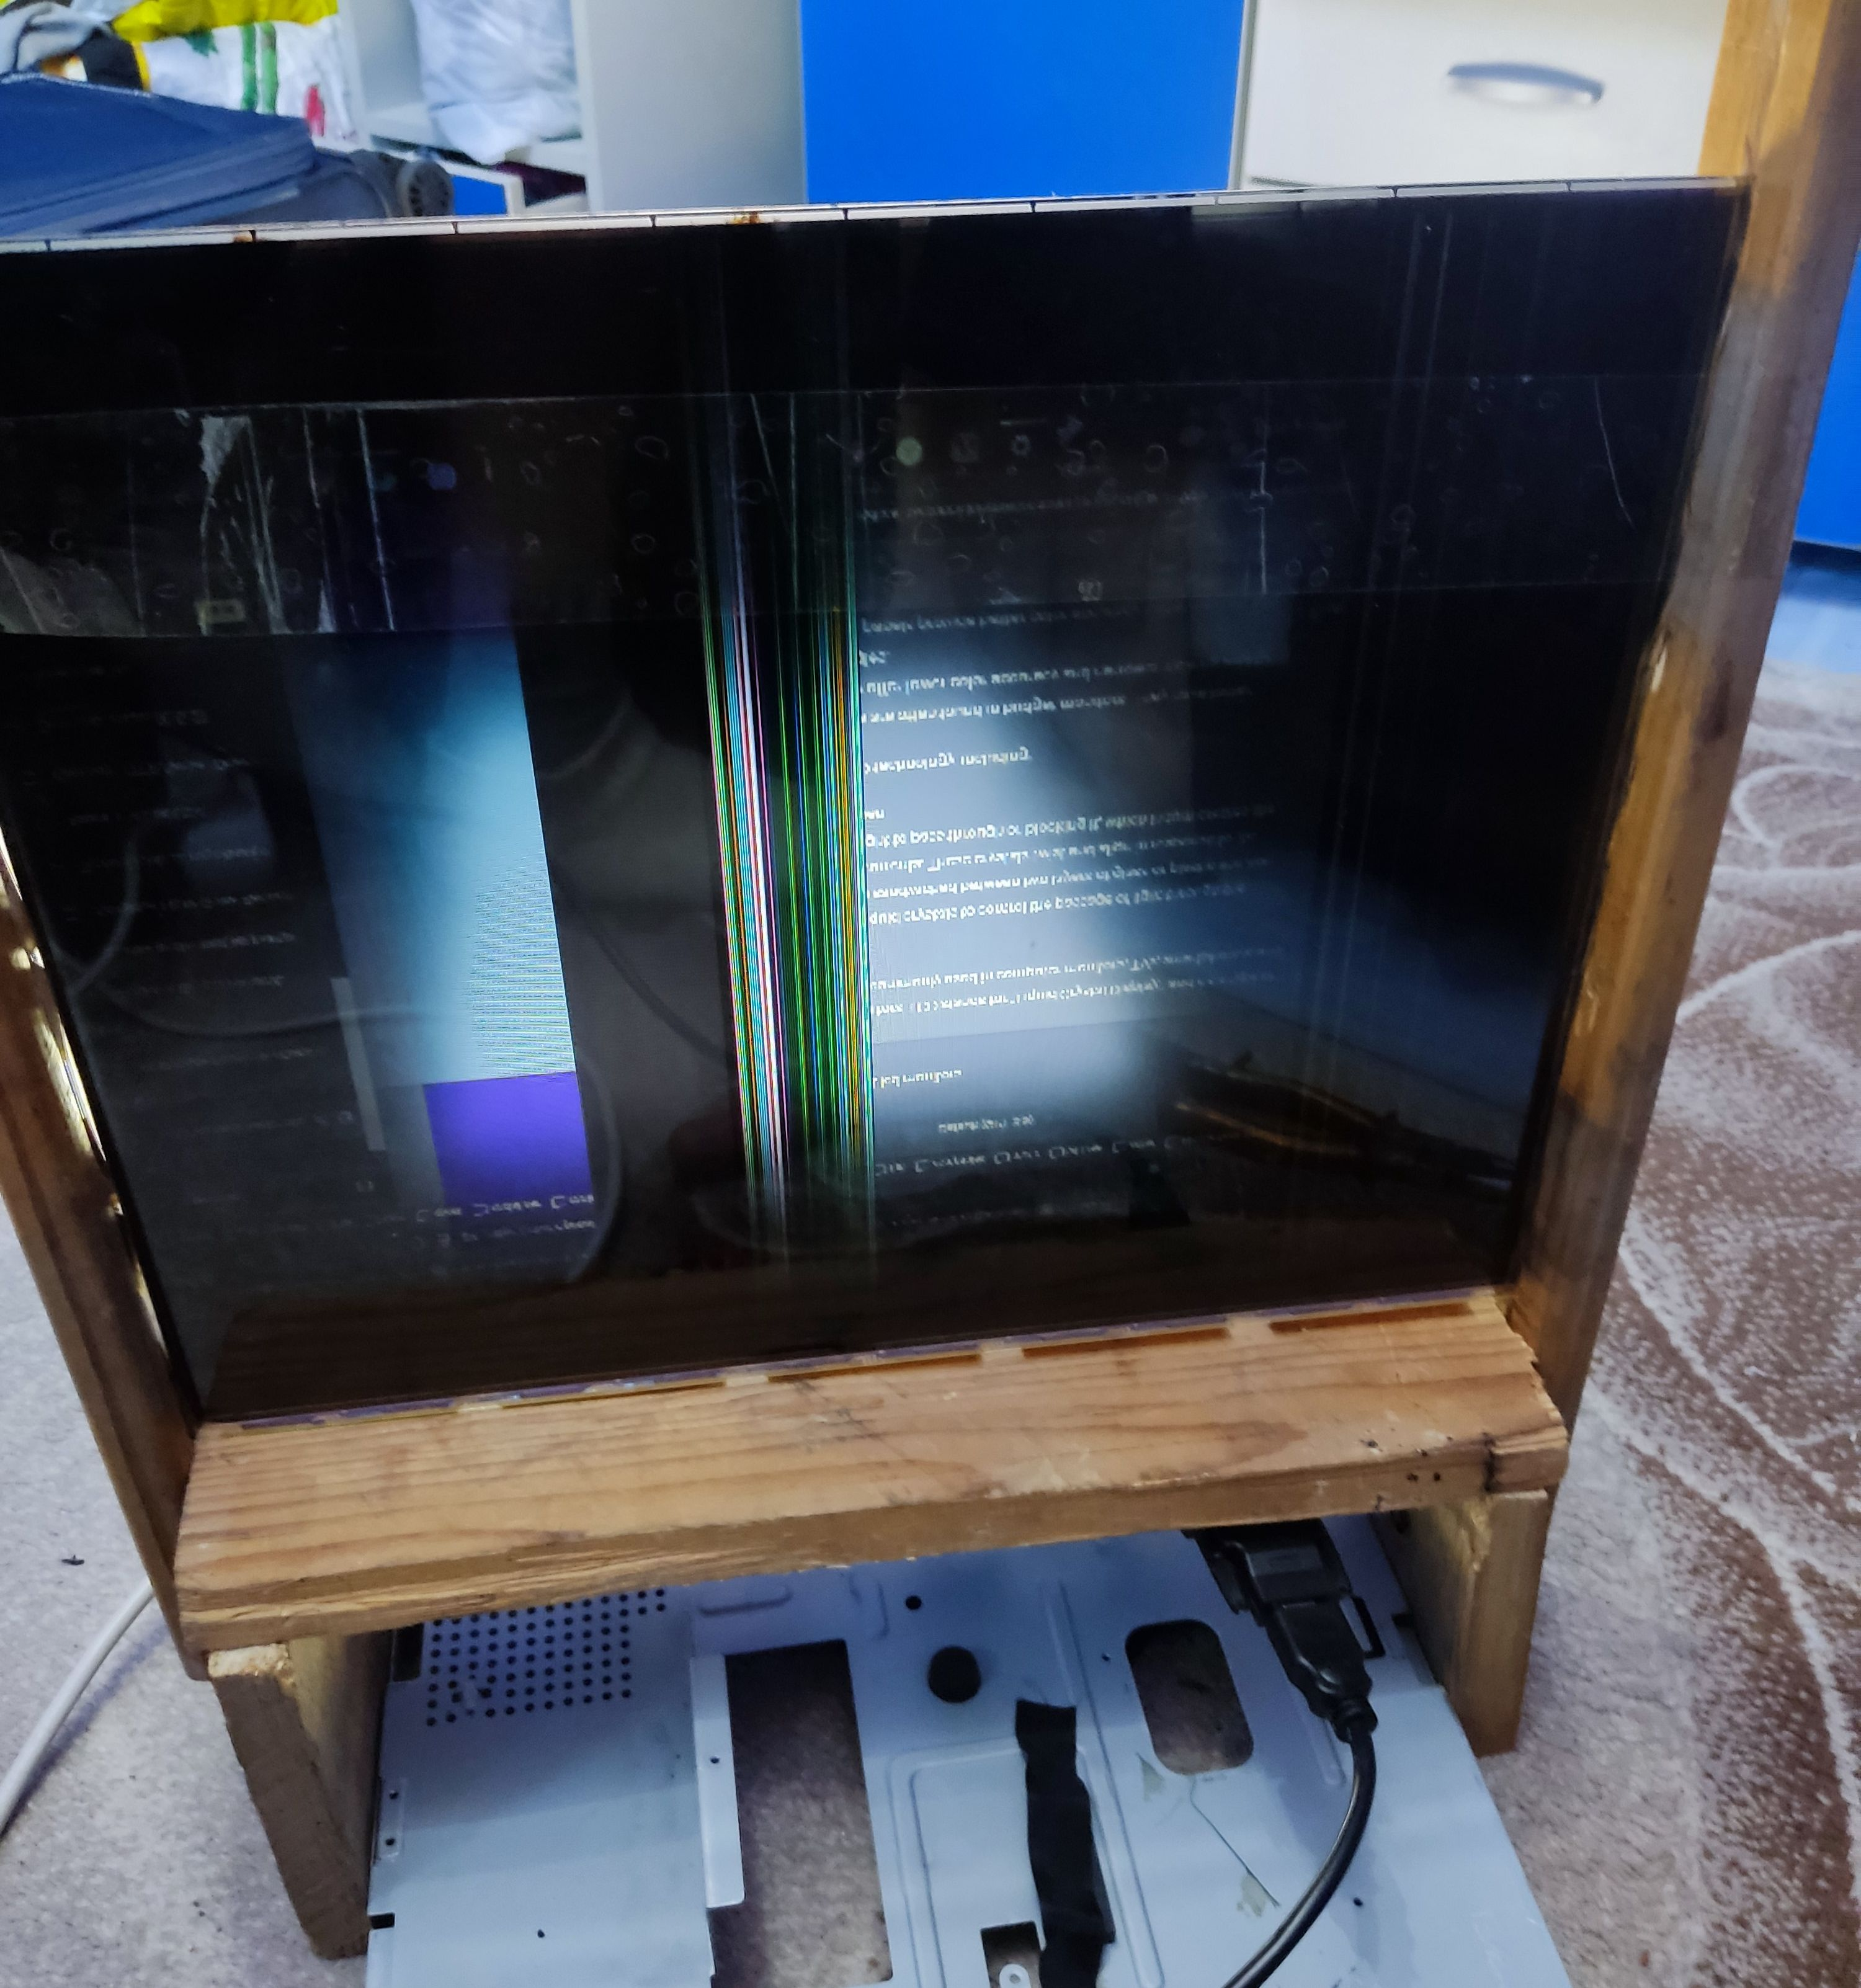
\includegraphics[width=0.5\textwidth]{slike/lcd_matrica_2}
    \captionsetup{font={small}}
    \caption{Prikaz LCD matrica sa zadnje strane kada je izvađena iz monitora [autorski rad]}
    \label{fig:lcd_matrica_2}
\end{figure}

TODO pronaći još jednu lcd matricu i pokušati s njom jer sam ovu pokvario :)

\subsection{OpenCV-Python biblioteka}

Budući da je potrebno prepoznati i pronaći točne pozicije na kojima se nalaze objekti od interesa odnosno svjetlost i oči, potrebno je koristiti algoritme za računalni vid. Kako IBM navodi (engl. \emph{International Business Machines Corporation - IBM}) \cite{cv-ibm}, računalni vid je grana umjetne inteligencija (engl. \emph{Artificial intelligence - AI}) koja omogućava računalima da pruže smislene informacije koje pronađu obradom slika, videa ili drugog vizualnog izvora te da reagiraju shodno toj informaciji. Zbog toga u ovom radu koristit će se biblioteka OpenCV za programski jezik Python.

OpenCV je biblioteka otvorenog koda (engl. \emph{open source}) koja služi za rješavanja problema vezanih za računalni vid (engl. \emph{computer vision}) i strojno učenje (engl. \emph{machine learning}) te pruža često potrebnu infrastrukturu za aplikacije koje integriraju računalni vid \cite{opencv}. OpenCV biblioteka podržava programske jezike C++, Python, Java, itd., i dostupna je na Windows, Linux, OS X, Andorid, iOS platformama. U radu će se koristiti OpenCV-Python biblioteka koja je Python API (engl. \emph{Application Programming Interface - API}) za OpenCV biblioteku koja uzima najbolje kvalitete OpenCV C++ API-ja i Python programskog jezika \cite{opencv-python}.

Programski jezik Python je izabran zbog osobnih preferencija autora. Treba se uzeti u obzir da je Python sporiji programski jezik u odnosu na C++ koji je se također mogao koristiti u ovom radu, no moguće je imati i Python module koji će sadržavati C++ programski kod za procesorski intenzivne zadatke, a rezultat toga je da se izvršavanja Python programskog koda izvršava približno jednakom brzinom kao i brzina izvršavanja C++ programskog koda jer se C++ kod izvršava u pozadini te lakše je programirati u Python programskom jeziku nego u C++ programskom jeziku \cite{opencv-python}.

Kako bi se koristila biblioteka OpenCV sa programskim jezikom Python potrebno ju je prvo instalirati. U terminalu unesite komandu: $pip$ $install$ $opencv-python$ i OpenCV biblioteka će biti instalirana. Ako ju želite korisiti u $conda$ radnom okruženju koje nudi dodatne pogodnosti slijediti upute za odgovarajući operativni sustav (OS) za:
\begin{itemize}[noitemsep]
    \item Linux OS: \url{https://youtu.be/gt0Mpi6FFzQ?si=QCLjiDrJcBCP5qV8},
    \item Windows OS: \url{https://youtu.be/RfFiTozvOdQ?si=6jtyHU4YK9jsi6kv},
    \item MacOS: \url{https://youtu.be/hZWgEPOVnuM?si=kD9CNUf4kNqyWBBK},
\end{itemize}
te je potrebno postaviti $conda$ radno okruženje: \url{https://www.jetbrains.com/help/pycharm/conda-support-creating-conda-virtual-environment.html}.

Nakon instalacije moguće je uključiti biblioteku pomoću sljedećeg programskog koda \ref{lst:lstlisting_1}:
\begin{lstlisting}[language=Python, label={lst:lstlisting_1}, firstnumber=1, style=colored, caption=Uključivanje biblioteke $OpenCV$]
import cv2 as cv
\end{lstlisting}

\justifying

\subsection{Redovi kao struktura podataka za spremanje okvira}

Ono što algoritam za računalni vid uzima kao ulazni podatak je fotografija odnosno okvir (engl. \emph{frame}) koji se dobiva od kamere koja cijelo vrijeme snima okolinu. Slika \ref{fig:slika_frame} objašnjava kako je skup okvira odnosno fotografija fotografiranih uzastopno u kratkom vremenskom periodu jednak videu te na taj način video i nastaje \cite{AnimoticaBlog2020}.

\begin{figure}[h!]
    \centering
    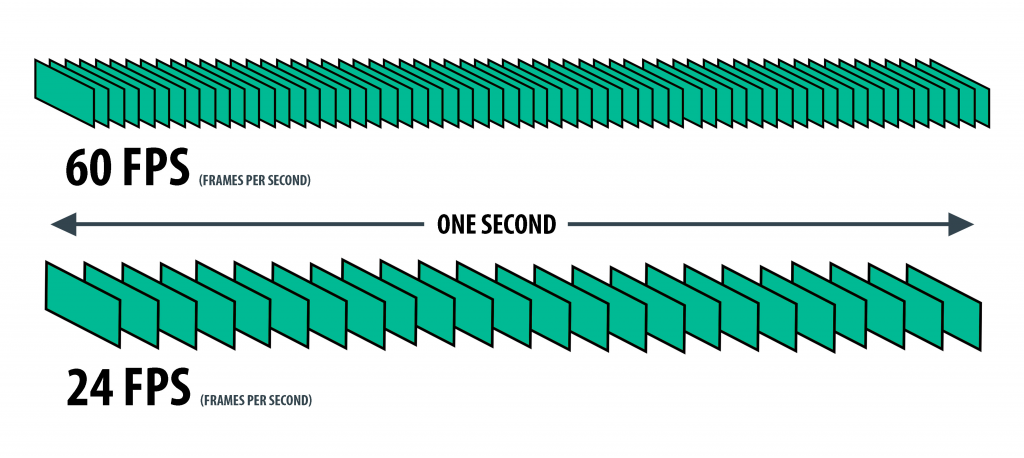
\includegraphics[width=1\textwidth]{slike/frames-per-second-diagram}
    \captionsetup{font={small}}
    \caption{Prikaz uzastopnih fotografija/okvira koji čine video od jedne sekunde \cite{AnimoticaBlog2020}}
    \label{fig:slika_frame}
\end{figure}

Budući da kamere cijelo vrijeme snimaju okolinu, one generiraju mnogo fotografiju u stvarnom vremenu od kojih će program uzimati po jednu fotografiju u određenom trenutku, analizirati ih i spremati ih u posebne strukture podataka za daljnju obradu. U ovom radu strukture podataka koje su uzete za ovu svrhu spremanja potrebnih informacija su redovi (engl. \emph{Queues}) tipa FIFO - "prvi ušao, prvi izašao" (engl. \emph{First In First Out - FIFO}).

Razlog zbog čega su odabrani redovi kao struktura podataka u koju će se spremati podaci je taj što redovi osiguravaju sigurno korištenje podataka između više dretava, a tip FIFO zbog toga što je bitno da se prvo analizira okvir koji je najprije došao \cite{PythonSoftwareFoundation}. To će biti vrlo korisno budući da će ovaj program koristiti glavnu dretvu za čitanje okvira iz redova i njihovo prikazivanje, i drugu dretvu za dobijanje okvira pomoću kamere, analiziranje i njihovo spremanje u redove. Slika \ref{fig:dijagram_red} slikovito prikaziva red kao strukturu podataka te prikaziva funkcije $get()$ i $put()$ klase $Queue$ pomoću kojih se podaci dodavaju i uzimaju iz redova. Programski kod \ref{lst:lstlisting_2} prikazuje kako uključiti biblioteku i inicijalizirati redove.

\begin{figure}[h!]
    \centering
    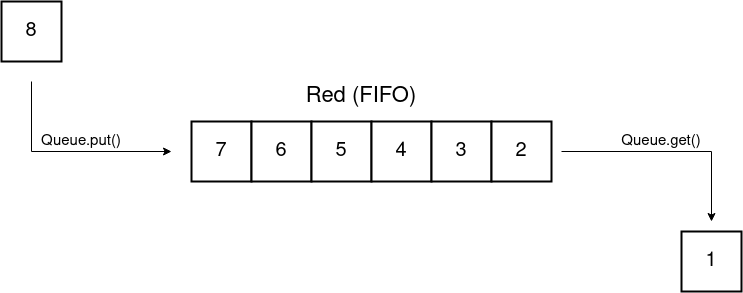
\includegraphics[width=0.7\textwidth]{slike/redovi_dijagram}
    \captionsetup{font={small}}
    \caption{Slikovit prikaz reda kao strukture podataka [autorski rad]}
    \label{fig:dijagram_red}
\end{figure}

\begin{lstlisting}[language=Python, label={lst:lstlisting_2}, firstnumber=4, style=colored, caption=Uključivanje biblioteke $queue$ i inicijaliziranje redova]
from queue import Queue

eyes_frames_queue = Queue()
light_frames_queue = Queue()

eyes_position_queue = Queue()
light_position_queue = Queue()
\end{lstlisting}

Programskim kodom \ref{lst:lstlisting_2} inicijalizirani su  $eyes\_frames\_queue$ i $light\_frames\_queue$ redovi koji služe za spremanje okvira koji se dobiju pomoću kamera i prikazivanje istih okvira nakon njihova analiziranja te još su inicijalizirani $eyes\_position\_queue$ i $light\_position\_queue$ redovi koji služe za spremanje koordinata za pozicije očiju i izvora svjetla koji se dobiju nakon analiziranja okvira i služe za kasnije računanje prilikom stvaranje sloja zaštite koji će se prikazivati na LCD matrici.

Okviri se prikazuju u posebno otvorenim prozorima na zaslonu laptopa i LCD matrice koje otvaramo sa programskim kodom \ref{lst:lstlisting_3}. Prvi prozor prikaziva okvire od kamere koja snima oči vozača, drugi prozor prikaziva okvire od kamere koja snima vanjsku okolinu koja dolazi ususret vozaču, a treći prozor je prozor koji će biti postavljen na LCD matricu i prikazivat će zaštitni okvir koji je ustvari okvir popunjen bijelom bojom, a crnom bojom na mjestima koja su izračunata kako bi se zatamnio određen dio matrice i spriječilo prodiranje svjetlosti. Kontinuirano prikazivanje okvira rezultira time da se može u realnom vremenu pratiti ono što kamere gledaju u obliku videa uživo (engl. \emph{live stream}).

\begin{lstlisting}[language=Python, label={lst:lstlisting_3}, firstnumber=142, style=colored, caption=Otvaranje prozora na zaslonu]
def open_window(name):
    cv.namedWindow(name, cv.WINDOW_NORMAL)
    cv.setWindowProperty(name, cv.WND_PROP_AUTOSIZE, cv.WINDOW_NORMAL)


if __name__ == '__main__':
win_name_eyes = 'Eyes Camera Preview'
open_window(win_name_eyes)

win_name_light = 'Light Camera Preview'
open_window(win_name_light)

win_name_protection = 'Protection Preview'
open_window(win_name_protection)
\end{lstlisting}

\subsection{Višedretvenost zbog raspodijele I/O zadataka}

\flushleft Zadatci koje program treba odrađivati su:
\begin{enumerate}[noitemsep]
    \item dohvačanje/čitanje okvira iz video izvora - ulaznog uređaja (kamere),
    \item analiziranje okvira (otkrivanje svjetlosti i očiju),
    \item spremanje pozicija i okvira u redove,
    \item čitanje okvira iz redova,
    \item izračunavanje pozicije koju treba zatamniti na LCD matrici,
    \item prikazivanje okvira u prozorima na zaslonu.
\end{enumerate}

\justifying

Navedeni zadatci su većinom vezani za ulazno/izlazne operacije (engl. \emph{input/output bound - I/O bound}) te ih je sve potrebno izvršavati istovremeno, zbog čega je korisno koristiti dretve kako bi se zadatci podijelili po dretvama koje možemo zamisliti kao dodatne radnike u firmi zbog kojih će se moći obaviti više posla paralelno s ostalim poslom. Dretve donose pojednostavljen dizajn koda i njihovo pravilno implementiranje ne može stvoriti situaciju da jedan zadatak zaustavlja izvođenje ostalih zadataka \cite{AndersonJim}.

U CPython implementaciji treba uzeti u obzir da se zbog GIL-a (engl. \emph{Global Interpreter Lock - GIL}) samo jedna dretva može izvršavati Python kod odjednom, a ovo se ograničenje može izbjeći korištenjem specijaliziranih biblioteka, no dojam paralelnosti se ipak postiže visokofrekventnom izmjenom rada nad dretvama. Dretve su prikladne za korištenje kod ulazno/izlaznih operacija, dok se kod procesorski složenijih zadataka savjetuje korištenje procesa \cite{PythonSoftwareFoundation2}. U ovom radu zadatci za analiziranje i izračunavanje nisu procesorski zahtjevni, stoga će ih dretve izvršavati.

\flushleft Potrebno je uključiti biblioteku pomoću sljedećeg programskog koda \ref{lst:lstlisting_thread}:
\begin{lstlisting}[language=Python, label={lst:lstlisting_thread}, firstnumber=2, style=colored, caption=Uključivanje biblioteke $threading$]
import threading
\end{lstlisting}

\justifying

Iz glavne dretve programa će se kreirati nova dretva koja će obavljati gore prva tri navedena zadatka: čitanje, analiziranje i spremanje pozicija i okvira, dok će glavna dretva obavljati gore zadnja tri navedena zadatka: čitanje, izračunavanje i prikazivanje pozicija i okvira. Programski kod \ref{lst:lstlisting_4} prikaziva definiranje i pokretanje nove dretve (153. do 157. linija koda) te pozivanje funkcije (159. linija koda) i inicijaliziranje dretvenog događaja (151. linija) na glavnoj dretvi koji će služiti za prekidanje čitanja okvira iz kamere na novoj dretvi. Kod stvaranja dretve definirana je funkcija koju ona treba izvršavati, proslijeđen joj je dretveni događaj kako bi ga mogla osluškivati i označena je kao $daemon$ dretva što znači da glavna dretva smije završiti iako ona nije završila. Dretveni događaji su mehanizmi komunikacije između dretava na način da jedna dretva može čekati postavljanje određenog događaja od strane druge dretve kako bi krenula sa svojim radom \cite{PythonSoftwareFoundation2}.

\begin{lstlisting}[language=Python, label={lst:lstlisting_4}, firstnumber=151, style=colored, caption={Inicijaliziranje dretvenog događaja $stop\_read\_event$, stvaranje i pokretanje nove dretve i pozivanje funkcije $read\_analyze\_and\_save\_frames()$ u glavnoj dretvi}]
stop_read_event = threading.Event()

threading.Thread(
    target=read_analyze_and_save_frames,
    args=(stop_read_event,),
    daemon=True
).start()

read_calculate_and_show_frames(win_name_eyes, win_name_light, win_name_protection)
\end{lstlisting}

\subsection{Kamere - čitanje okvira s video izvora}

Kako bi se u realnom vremenu moglo otkriti zasljepljujeće svjetlo i oči u cilju smanjivanja zasljepljujećg svjetla potrebno je cijelo vrijeme neprekidno pratiti sadržaj onoga što kamere vide odnosno čitati okvire sa video izvora. Podsjetnik - jedan pročitan okvir je ustvari jedna fotografija iz videa. Porgramski kod \ref{lst:lstlisting_5} prikazuje definiciju $read\_analyze\_and\_save\_frames()$ funkcije koja se izvršava na posebnoj novoj dretvi, a iz definicije funkcije može se vidjeti kako isprogramirati čitanje okvira sa video izvora.

\begin{lstlisting}[language=Python, label={lst:lstlisting_5}, firstnumber=13, style=colored, caption={Definicija funkcije $read\_analyze\_and\_save\_frames()$}]
def read_analyze_and_save_frames(stop_event):
    camera_indexes = [0, 2]

    eyes_source = cv.VideoCapture(camera_indexes[0])
    light_source = cv.VideoCapture(camera_indexes[1])

    while not stop_event.is_set():
        has_eye_frame, eyes_frame = eyes_source.read()
        has_light_frame, light_frame = light_source.read()

        if not has_eye_frame or not has_light_frame:
            print("Frame not found. Check cameras.\n")
            break

        detect_eyes(eyes_frame)
        detect_light(light_frame)

    eyes_source.release()
    light_source.release()
\end{lstlisting}

Potrebno je inicijalizirati video izvore na način da se pronađu odgovarajući indeksi za kamere koje će se koristiti. U ovom radu, index za ugrađenu kameru laptopa je $0$, dok je za eksternu kameru indeks $2$ (14. linija koda). Kada su uspješno identificirani indeksi za kamere moguće je inicijalizirati video izvore korištenjem klase $VideoCapture$ iz OpenCV biblioteke koja omogućava video snimanje iz kamera i dodatno je moguće snimati iz video datoteka i nizova fotografija/okvira \cite{OpenCV2} (16. i 17. linija koda). Čitanje iz nizova okvira će se koristiti u ovom radu prilikom prikazivanja okvira gdje će se okviri čitati iz redova $eyes\_frames\_queue$ i $light\_frames\_queue$. Nakon prestanka korištenja video izvora potrebno je video izvore otpustiti (30. i 31. linija koda).

Nakon što su video izvori  inicijalizirani moguće je čitati okvire iz njih. Kako bi cijelo vrijeme neprekidno čitali jedan po jedan okvir sa kamere i prikazivali ih u stvarnom vremenu, potrebno je koristiti $while$ $True$ petlju. U ovom radu koristi se $while$ $not$ $stop\_event.is\_set()$ petlja (19. linija koda) kod koje je izraz $not stop\_event.is\_set()$ uvijek jednak Booleovoj vrijednosti $True$, zbog čega će se stalno izvršavati dok događaj $stop\_event$ koji je kao argument proslijeđen u $read\_analyze\_and\_save\_frames()$ funkciju ne bude postavljen na $True$ u slučaju kada korisnik želi prekinuti program.

Okvir se čita sa metodom $read()$ iz klase $VideoCapture$ (20. i 21. linija koda), a ona objedinjuje metode $grab()$ i $retrieve()$ te dekodira vrijednost okvira \cite{OpenCV2}. Metoda $read()$ vraća informacije o tome je li okvir uspješno pročitan i njegovu vrijednost, a njegova vrijednost je u formi $NumPy$ niza \cite{Reshma2023}. Na slici \ref{fig:ispis_okvira} može se vidjeti da taj NumPy niz sadrži cjelobrojne vrijednosti (engl. \emph{integers}) koje predstavljaju RGB vrijednosti kanala piksela sa fotografije odnosno okvira. NumPy biblioteka služi za rad sa nizovima \cite{NumPy}. Ako okvir nije uspješno pročitan, prekida se izvođenje petlje (23. do 25. linija koda).

\begin{figure}[h!]
    \centering
    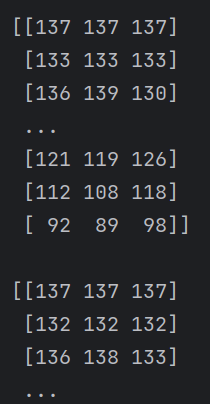
\includegraphics[width=0.2\textwidth]{slike/numpy_frame}
    \captionsetup{font={small}}
    \caption{Ispis dijela vrijednosti za okvir koju vrati $cv::VideoCapture::read$ metoda [autorski rad]}
    \label{fig:ispis_okvira}
\end{figure}

U svakom krugu petlje čita se po jedan okvir i odmah se taj okvir analizira funkcijama $detect\_eyes()$ i $detect\_light()$ kako bi se otkrila pozicija zasljepljujućeg svjetla i očiju (27. i 28. linija koda). Funkcije $detect\_eyes()$ i $detect\_light()$ predstavljaju komponente sustava koje su obrađene u sljedećim poglavljima: "Komponenta za prepoznavanje i pozicioniranje izvora svjetla" i "Komponenta za prepoznavanje i pozicioniranje očiju vozača".

Slika \ref{fig:sustav1} prikaziva kako okviri izgledaju prije otkrivanja zasljepljujućeg svjetla i očiju. Na zaslonu ne trebaju biti otvoreni prikazani prozori sa slike \ref{fig:sustav1}, ali su tu samo kako bi se uvidjelo da sustav odrađiva ono što treba i kako bi se bolje shvatilo kako sustav radi.

\begin{figure}[h!]
    \centering
    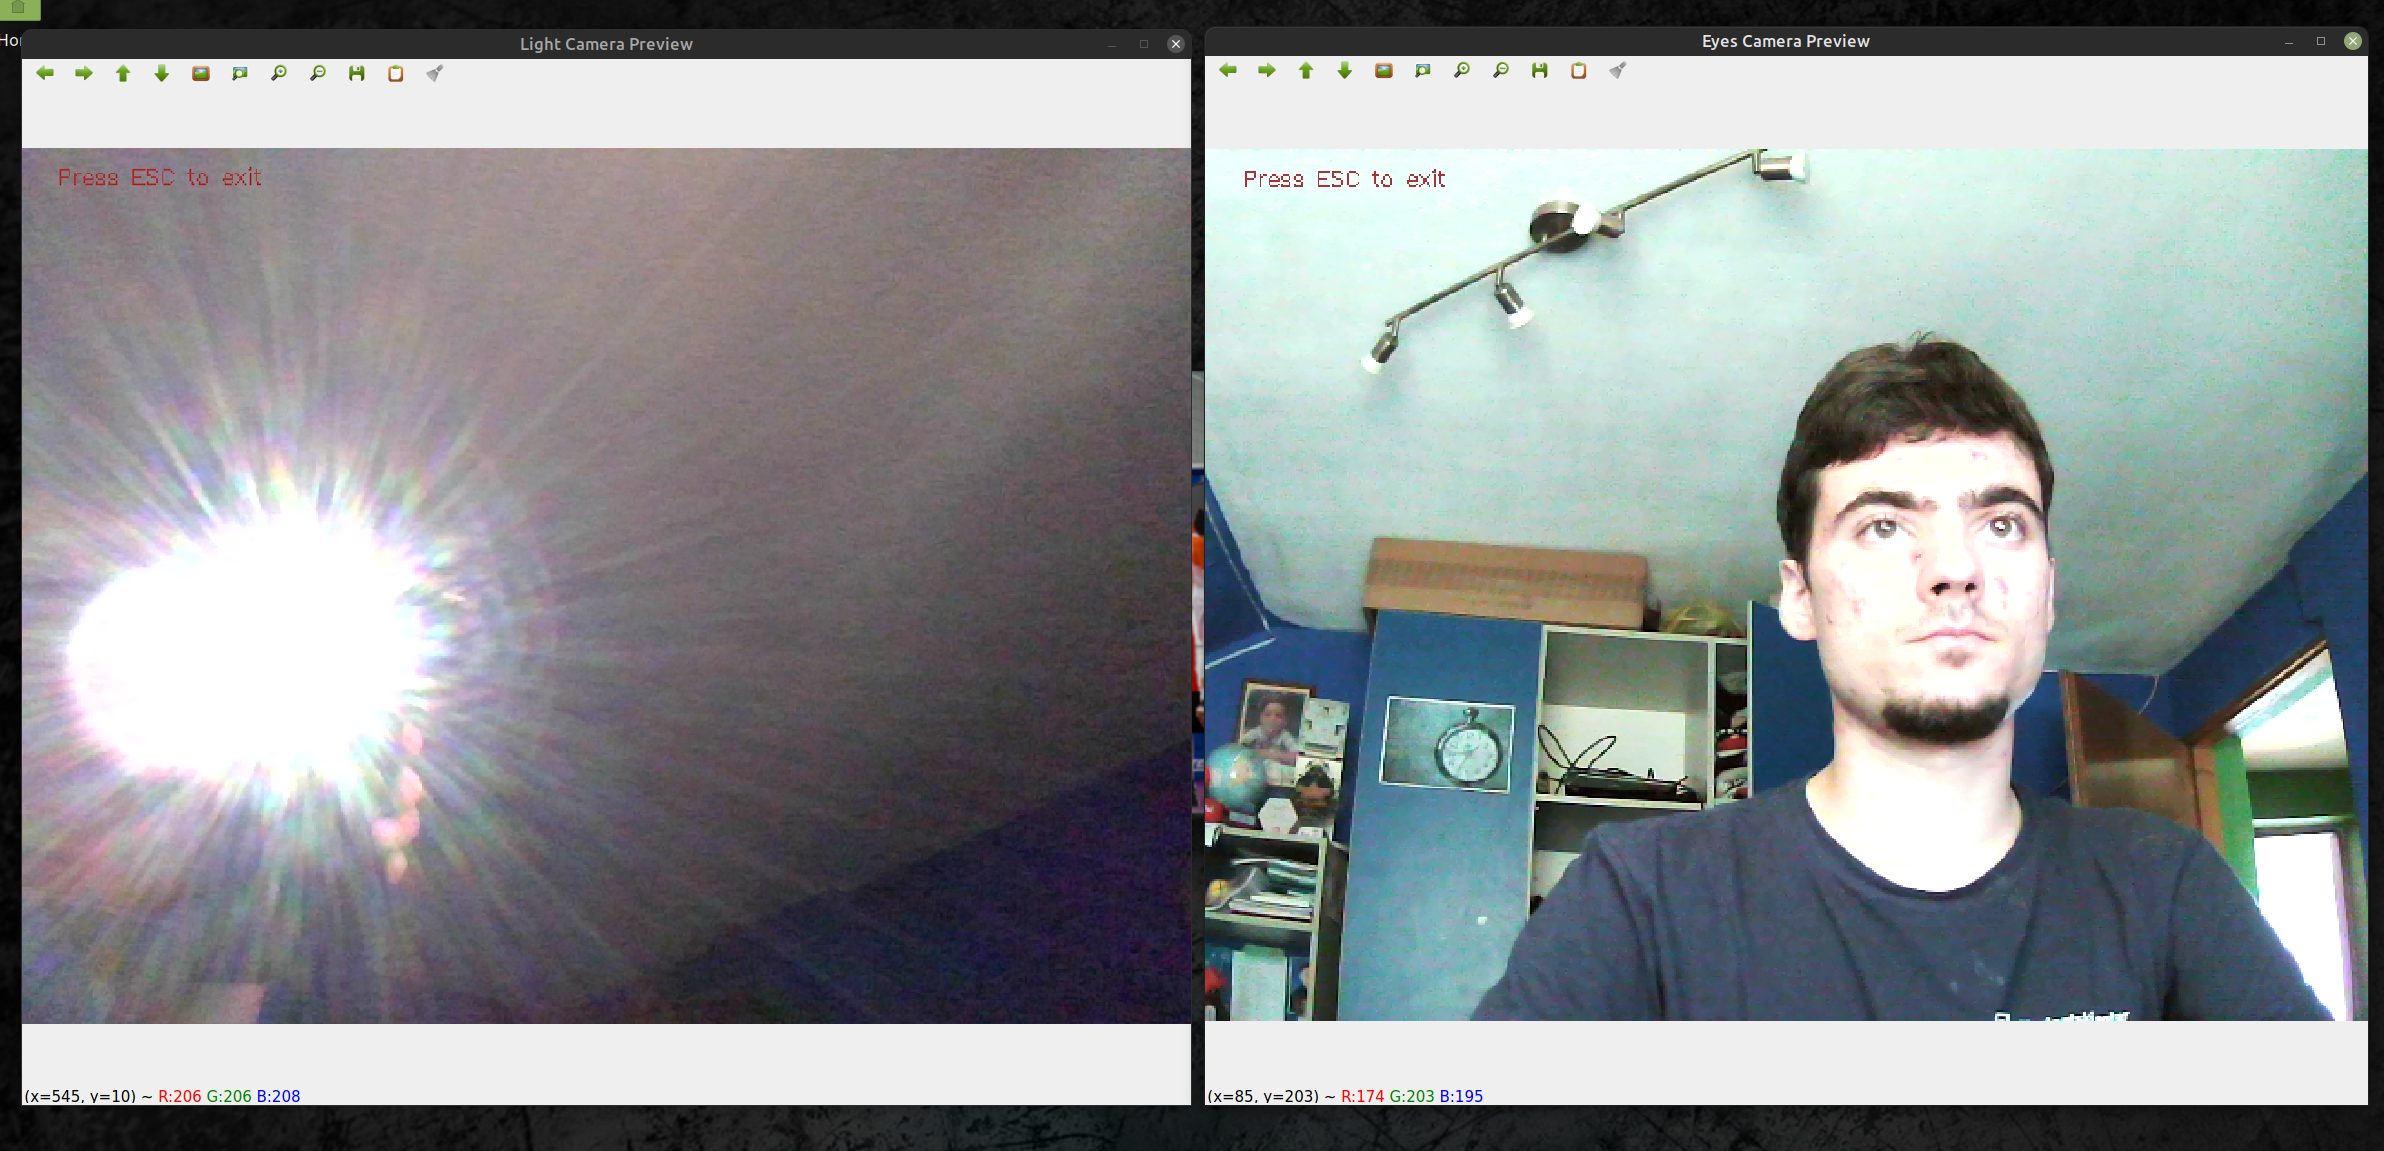
\includegraphics[width=1\textwidth]{slike/sustav1}
    \captionsetup{font={small}}
    \caption{Prikaz okvira prije otkrivanja zasljepljujućeg svjetla i očiju [autorski rad]}
    \label{fig:sustav1}
\end{figure}

\pagebreak
\section{Komponenta za prepoznavanje i pozicioniranje izvora svjetla}

Nakon što se uspješno čitaju okviri s kamere koja gleda okolinu koja je ispred vozača, potrebno je analizirati svaki okvir i otkriti nalazi li se na njima zasljepljujuća svjetlost. Ako se svjetlost nalazi na okviru, potrebno je pronaći točne koordinate svjetlosti na okviru. Ovo poglavlje će kroz programski kod \ref{lst:lstlisting_6} koji prikaziva definiranje funkcije $detect\_light()$ za otkrivanje zasljepljujuće svjetlosti opisati navedeni potrebni zadatak.

\flushleft Potrebno je uključiti biblioteku pomoću sljedećeg programskog koda \ref{lst:lstlisting_numpy}:
\begin{lstlisting}[language=Python, label={lst:lstlisting_numpy}, firstnumber=3, style=colored, caption=Uključivanje biblioteke $numpy$]
import numpy as np
\end{lstlisting}

\begin{lstlisting}[language=Python, label={lst:lstlisting_6}, firstnumber=50, style=colored, caption={Definicija funkcije $detect\_light()$}]
def detect_light(light_frame):
    lower_range = np.array([0, 0, 255])
    upper_range = np.array([240, 11, 255])

    light_hsv_frame = cv.cvtColor(light_frame, cv.COLOR_BGR2HSV)

    color_mask = cv.inRange(light_hsv_frame, lower_range, upper_range)

    contours, _ = cv.findContours(color_mask, cv.RETR_EXTERNAL, cv.CHAIN_APPROX_SIMPLE)

    min_contour_area = 4000
    big_contours = [contour for contour in contours if cv.contourArea(contour) > min_contour_area]

    light_positions = []

    for contour in big_contours:
        light_positions.append(cv.boundingRect(contour))

        x, y, w, h = cv.boundingRect(contour)
        cv.rectangle(light_frame, (x, y), (x + w, y + h), (0, 255, 0), 2)

    light_position_queue.put(light_positions)

    drawText(light_frame, 'Press ESC to exit', (20, 20))

    light_frames_queue.put(light_frame)
\end{lstlisting}

\justifying

Idealno bi bilo kada bi ovakvo rješenje mogli kombinirati i sa senzorom koji može izmjeriti intenzitet svjetlosti jer bi se mogla otkriti i zasljepljujuća svjetlost drugih boja osim raspona bijele boje koji je jedini definiran u ovom rješenju za otkrivanje zasljepljujuće svjetlosti te također bi se svjetlost mogla lakše klasificirati. U programskom kodu \ref{lst:lstlisting_6} definiran je raspon bijele boje koji će se otkrivati na okviru (51. i 52. linija koda). Bijela boja je izabrana zato što je svjetlost najčešće bijele do žute boje.

Kao argument ova funkcija prima okvir koji treba analizirati. Potrebno je tom okviru promijeniti prostor boja (engl. \emph{color space}) iz BGR prostora boja (engl. Blur-Green-Red - BGR; OpenCV koristi BGR prostor boja umjesto RGB prostora boja zbog toga što je prilikom početnih godina OpenCV-a BGR prostor boja bio dosta popularniji kod proizvođača kamera i pružatelja softvera, a tako je i ostalo do danas \cite{Satya}) u HSV prostor boja (54. linija koda) zbog toga što funkcija $inRange()$ biblioteke OpenCV koristi HSV prostor boja te ona će kao argumente primiti originalni okvir i raspon boja. Funkcijom $inRange()$ dobit ćemo masku okvira popunjenu crno-bijelom bojom gdje bijela boja predstavlja objekt od interesa koji se svojom bojom nalazi u definiranom rasponu boje \cite{OpenCV3} (56. linija koda). Na slici \ref{fig:maska} možete vidjeti kako je funkcija $inRange()$ stvorila masku okvira sa crnom i bijelom bojom gdje bijela boja predstavlja zasljepljujuću svjetlost:

\begin{figure}[h!]
    \centering
    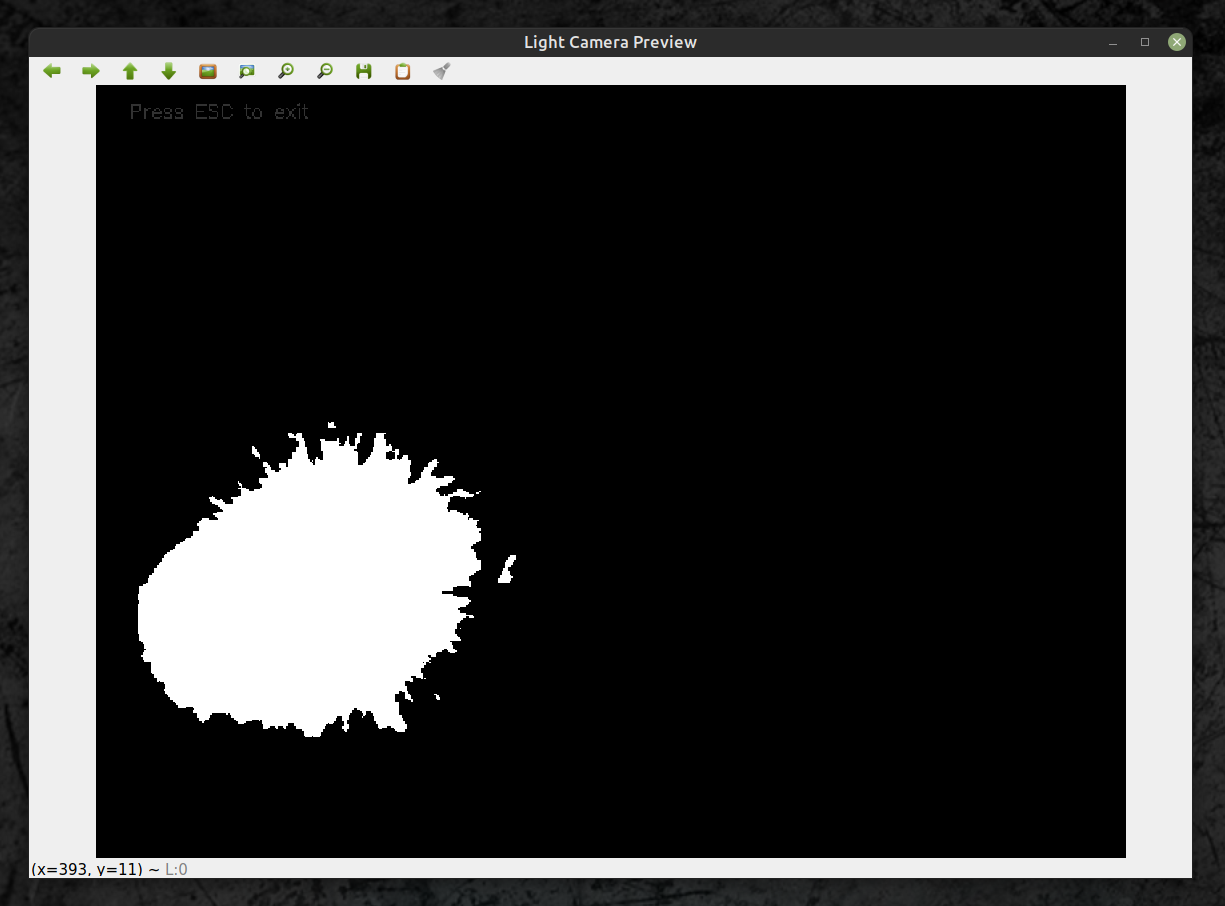
\includegraphics[width=0.6\textwidth]{slike/cb_maska_okvir}
    \captionsetup{font={small}}
    \caption{Prikaz crno-bijele maske okvira [autorski rad]}
    \label{fig:maska}
\end{figure}

Sada se može reći da je zasljepljujuća svjetlost otkrivena, ali se ne zna njezina točna pozicija s koordinatama što će poslužiti kod obavljanja računanja zaštitnog okvira za LCD matricu. Stoga svo ovo provedeno pretvaranje okvira je učinjeno zbog toga što će maska okvira biti proslijeđena funkciji $findContours()$ biblioteke OpenCV koja još prima argumente $cv.RETR\_EXTERNAL$ i $cv.CHAIN\_APPROX\_SIMPLE$ koji definiraju kakve će se konture praviti (58. linija koda). U ovom rješenju kontura predstavlja pravokutnik koji obuhvaća objekt od interesa i za taj pravokutnik dobijemo koordinate gornje lijeve točke, visinu i širinu. Funkcija $findContours()$ nije obavezno tražila svo provedeno pretvaranje okvira ali zbog boljeg pronalska kontura preporučeno je da funkcija primi binarni okvir - crno-bijelu masku kako bi rubovi bili što izraženiji \cite{OpenCV4}. Kako bi samo imali konture najizraženijih i najvećih svjetlosti odrađeno je i filtriranje (60. i 61. linija koda).

Sada je potrebno proći kroz svaku pronađenu konturu kako bi ju dodali u $light\_position\_queue$ red i kako bi na originalnom okviru iscrtali zeleni pravokutnik oko zasljepljujuće svjetlosti i spremili originalni okvir u $light\_framesq\_queue$ red (63. do 75. linija koda). Potrebno je naglasiti da pralaleno radi i glavna dretva koja odmah uzima okvire stavljene u red i prikaziva ih u prozorima na zaslonu, a o tome će biti više rijeći u poglavlju "Komponenta za polarizaciju LCD matrice kao reaktivne komponente". Iscrtavanje zelenog pravokutnika na originalnom okviru (slika \ref{fig:sustav2}) napravljeno je samo zbog toga kako bi se uvjerili da otkrivena zasljepljujuće svjetlosti radi:

\begin{figure}[h!]
    \centering
    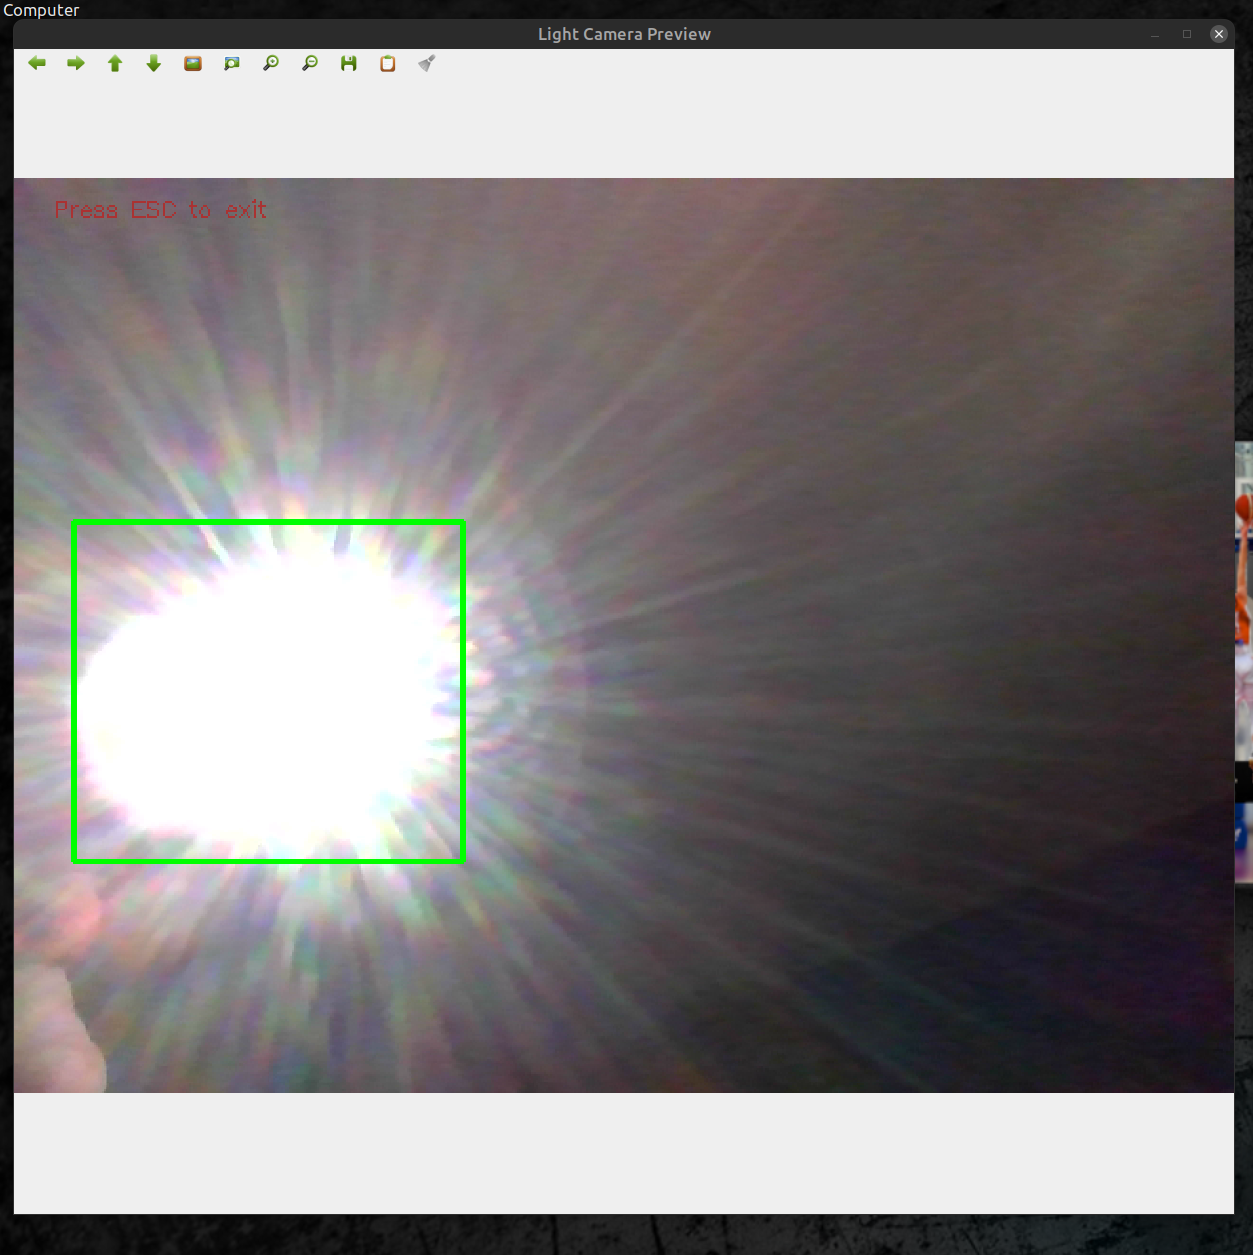
\includegraphics[width=0.6\textwidth]{slike/sustav2}
    \captionsetup{font={small}}
    \caption{Prikaz otkrivene svjetlosti [autorski rad]}
    \label{fig:sustav2}
\end{figure}

\pagebreak
\section{Komponenta za prepoznavanje i pozicioniranje očiju vozača}

Nakon što se uspješno čitaju okviri s kamere koja gleda u vozača, potrebno je analizirati svaki okvir i otkriti nalaze li se na njima oči. Ako se oči nalaze na okviru, potrebno je pronaći točne koordinate očiju na okviru. Ovo poglavlje će kroz programski kod \ref{lst:lstlisting_9} koji prikaziva definiranje funkcije $detect\_eyes()$ za otkrivanje očiju opisati navedeni potrebni zadatak.

\begin{lstlisting}[language=Python, label={lst:lstlisting_9}, firstnumber=33, style=colored, caption={Definicija funkcije $detect\_eyes()$}]
def detect_eyes(eyes_frame):
    eyes_gray_frame = cv.cvtColor(eyes_frame, cv.COLOR_BGR2GRAY)

    eye_cascade_model = cv.CascadeClassifier(cv.data.haarcascades + 'haarcascade_eye.xml')

    eyes = eye_cascade_model.detectMultiScale(eyes_gray_frame, scaleFactor=1.1, minNeighbors=5, minSize=(30, 30))

    eyes_position_queue.put(eyes)

    for (x, y, w, h) in eyes:
        cv.rectangle(eyes_frame, (x, y), (x + w, y + h), (0, 255, 0), 2)

    drawText(eyes_frame, 'Press ESC to exit', (20, 20))

    eyes_frames_queue.put(eyes_frame)
\end{lstlisting}

Otkrivanje očiju se vrši pomoću OpenCV klase $CascadeClassifier$ koja je model za otkrivanje objekata pomoću Haar kaskadnih klasifikatora, a to je pristup temeljen na strojnom učenju gdje je je kaskadna funkcija trenirana na mnogo pozitivnih (sadržavaju objekt od interesa) i negativnih fotografija (ne sadržavaju objekt od interesa) \cite{OpenCV5}. Prije nego se krene analizirati okvir, preporučeno je zbog boljih rezultata da se okvir prebaci u sivi prostor boja (34. linija koda).

Prilikom inicijaliziranja objekta klase $CascadeClassifier$ navodi se što je objekt od interesa - ovdje je to oko (36. linija koda). Kada je objekt inicijaliziran možemo njegovoj metodi $detectMultiScale$ proslijediti okvir koji se treba analizirati te je još moguće proslijediti argumenata koji bi utjecali na rezultat. Kao rezultat metoda vraća otkrivene objekte različitih veličina u obliku liste pravokutnika koji opisuju točnu poziciju (koordinate gornjeg lijevog kuta pravokutnika na okviru te njegova duljina i širina) očiju na okviru \cite{OpenCV6}. Lista pravokutnika se sprema u $eyes\_position\_queue$ red za daljno računanje (40. linija koda), a još će se i lista pravokutnika iscrtati na originalnim okvirima i spremiti u $eyes\_frames\_queue$ red kako bi prilikom prikazivanja okvira uvidjeli da komponenta pravilno radi (slika \ref{fig:sustav3}).

\begin{figure}[h!]
    \centering
    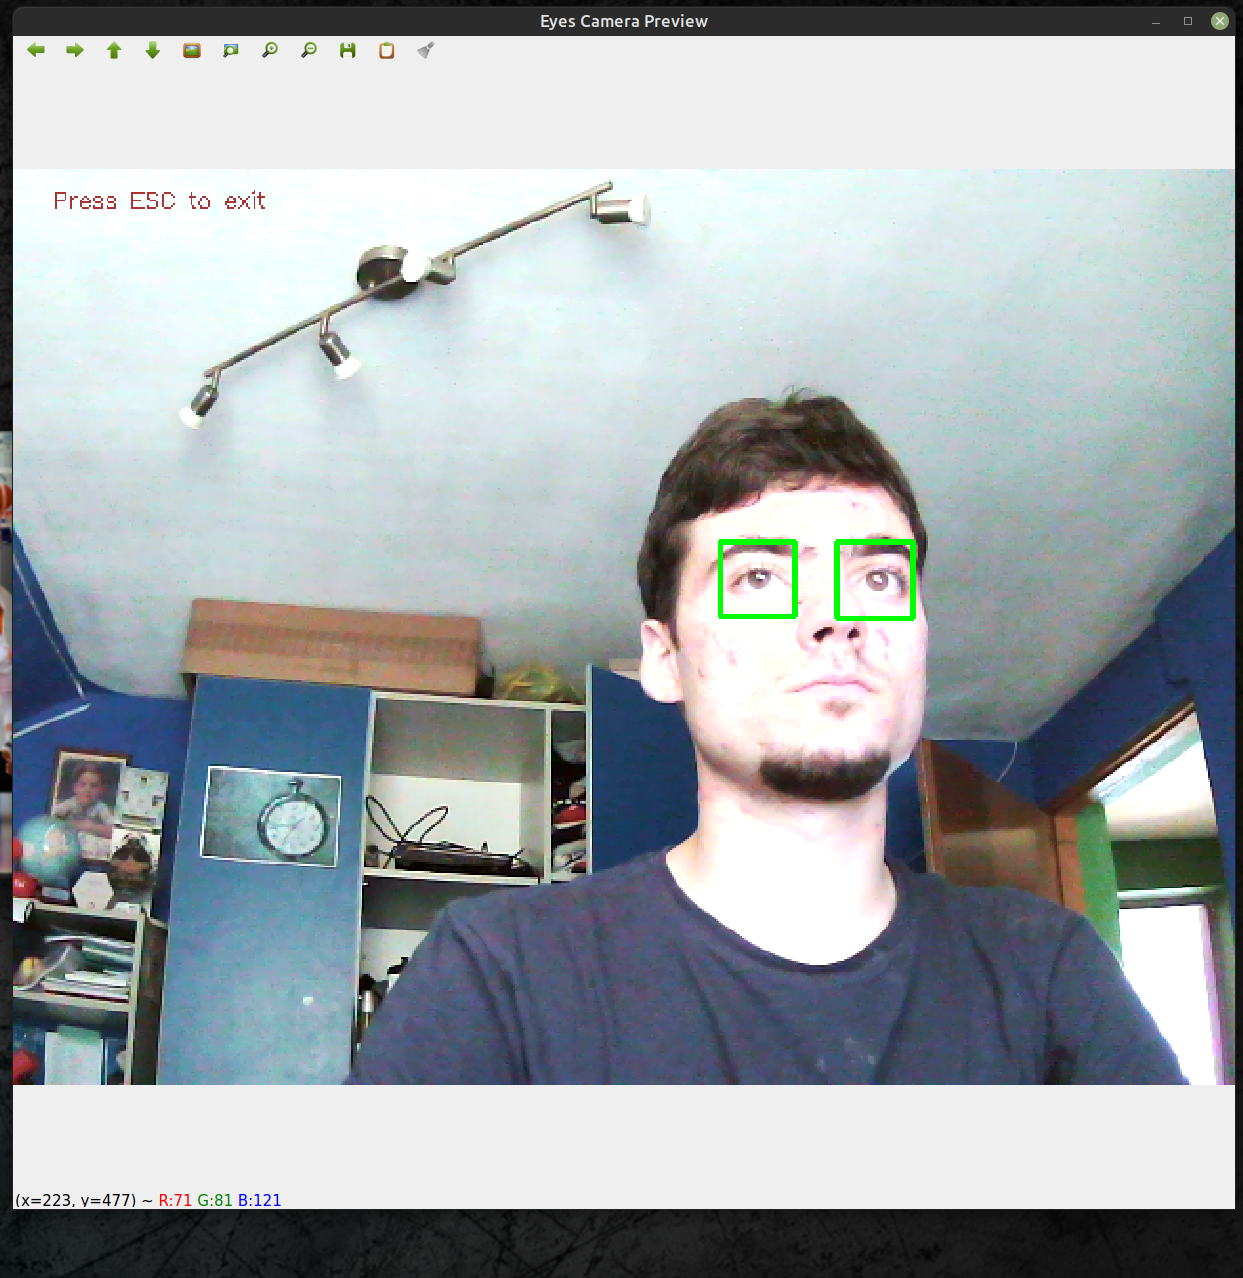
\includegraphics[width=0.6\textwidth]{slike/sustav3}
    \captionsetup{font={small}}
    \caption{Prikaz otkrivenih očiju [autorski rad]}
    \label{fig:sustav3}
\end{figure}

\pagebreak
\section{Komponenta za polarizaciju LCD matrice kao reaktivne komponente}

Kada su pozicije zasljepljujućeg svjetla i očiju poznate, potrebno je izračunati na kojem mjestu treba zatamniti LCD matricu, a selektivno zatamnjivanje matrice ustvari znači postavljanje na crnu boju jednog dijela novog zaštitnog okvira koji će se prikazivati u prozoru na LCD matrici. Kako bi se bolje shvatila problematika, sljedeće slike \ref{fig:sustav5} i \ref{fig:sustav6} prikazuju pojednostavljen prikaz sustava u trodimenzionalnom koordinatnom sustavu sa jednakom udaljenosti od matrice.

\begin{figure}[h!]
    \centering
    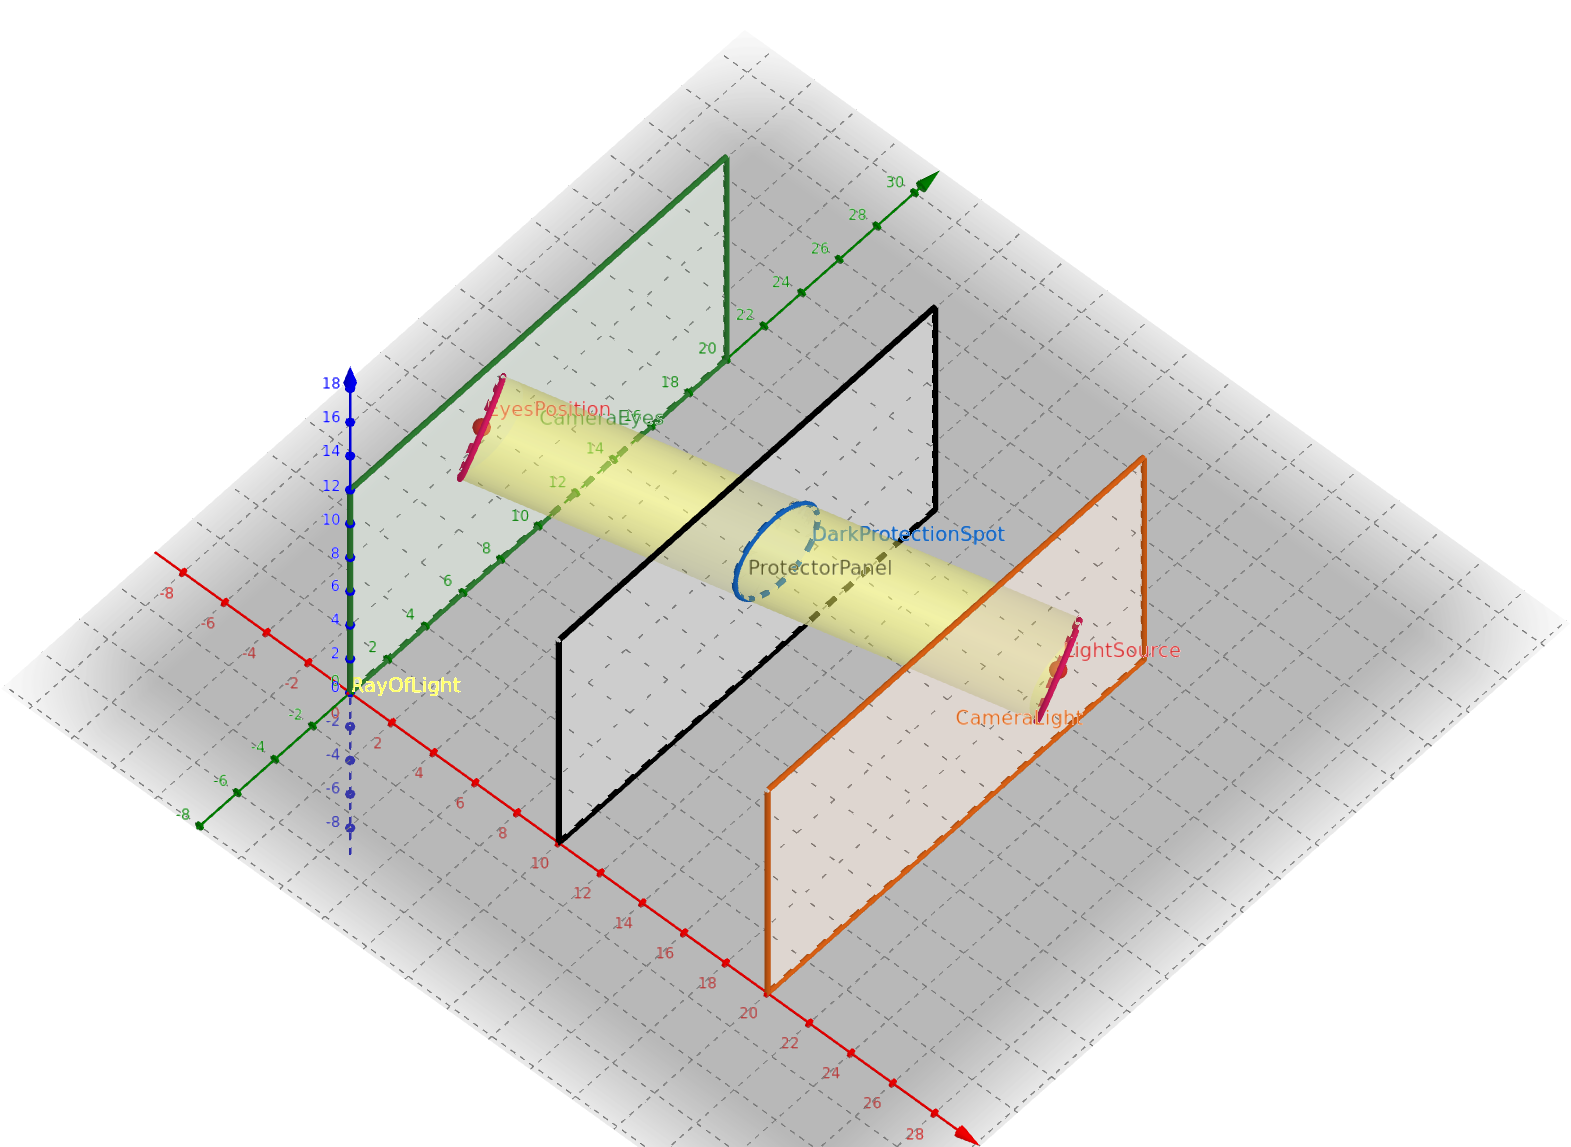
\includegraphics[width=0.8\textwidth]{slike/sustav5}
    \captionsetup{font={small}}
    \caption{Pojednostavljen prikaz sustava u trodimenzionalnom koordinatnom sustavu sa jednakom udaljenosti od matrice [autorski rad]}
    \label{fig:sustav5}
\end{figure}

\begin{figure}[h!]
    \centering
    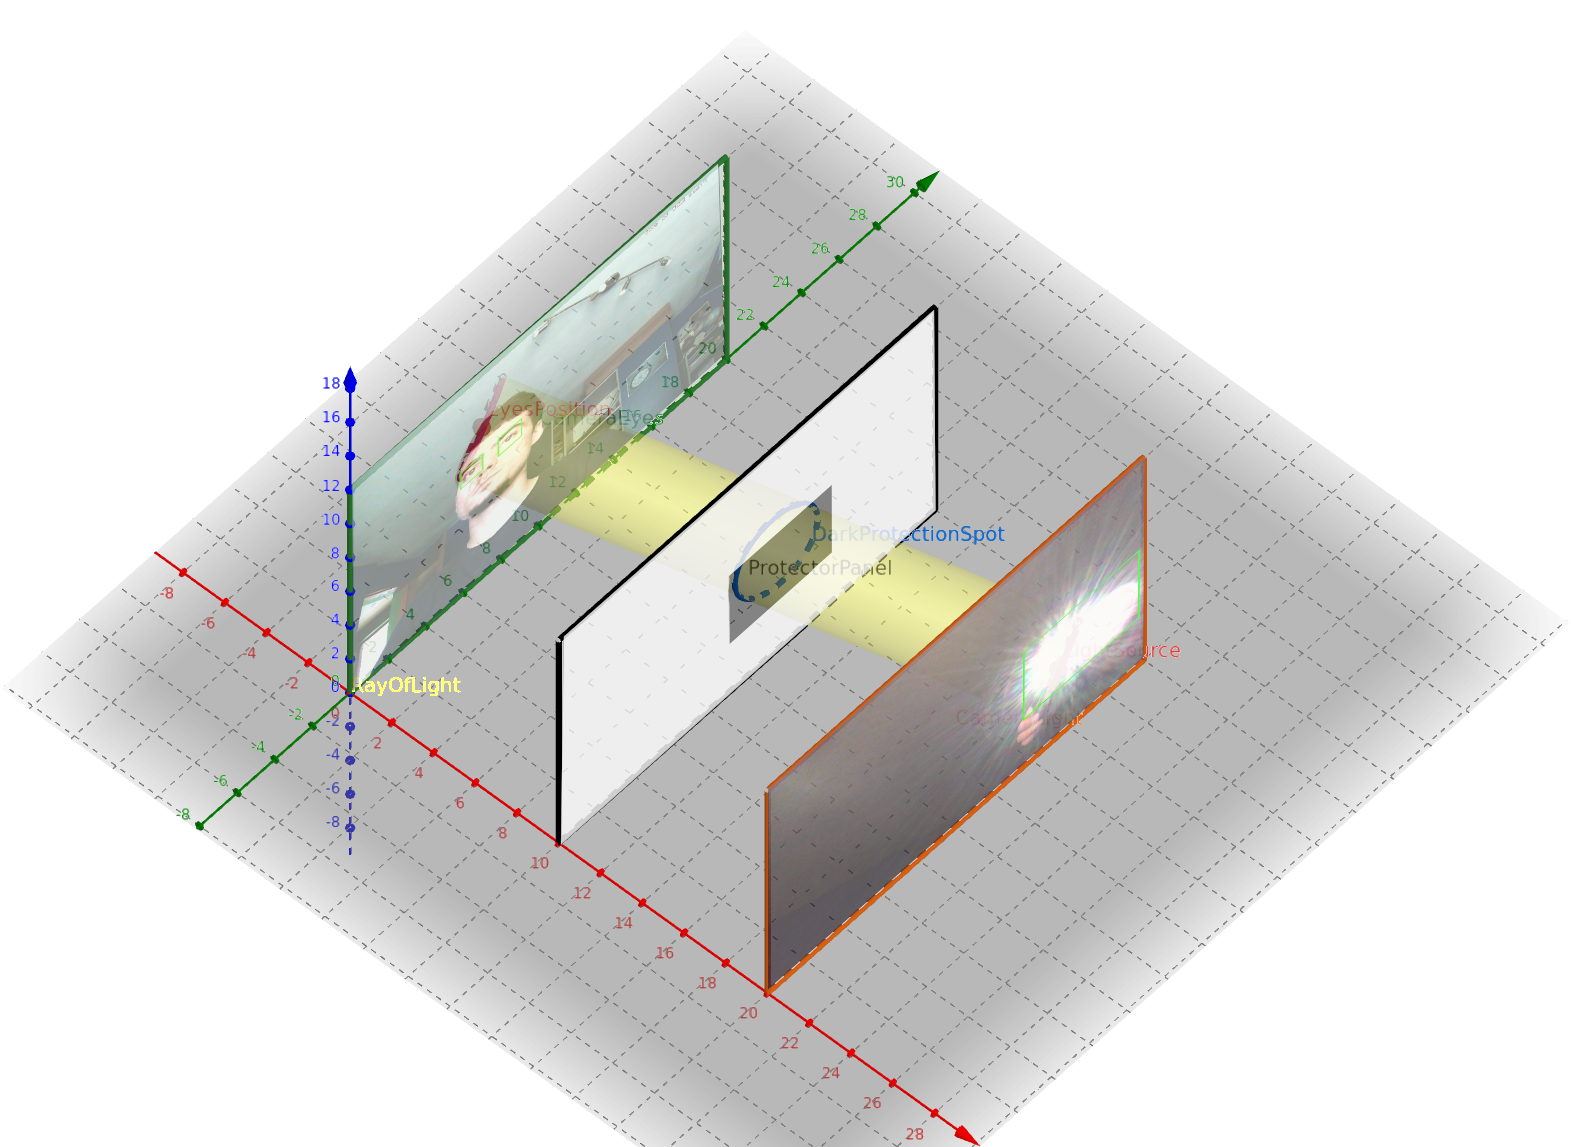
\includegraphics[width=0.8\textwidth]{slike/sustav6}
    \captionsetup{font={small}}
    \caption{Pojednostavljen prikaz sustava sa simbolično prikazanim okvirima u trodimenzionalnom koordinatnom sustavu sa jednakom udaljenosti od matrice [autorski rad]}
    \label{fig:sustav6}
\end{figure}

Zbog jednostavnosti izračuna, zamišljena udaljenost vozača od LCD matrice i udaljenost zasljepljujućeg svjetla od LCD matrice uzeta je kao jednaka.

Sljedeća slika \ref{fig:sustav4} prikaziva kako ovaj graf izgleda iz druge perspektive, odnosno u dvodimenzionalnom koordinatnom sustavu.

\begin{figure}[h!]
    \centering
    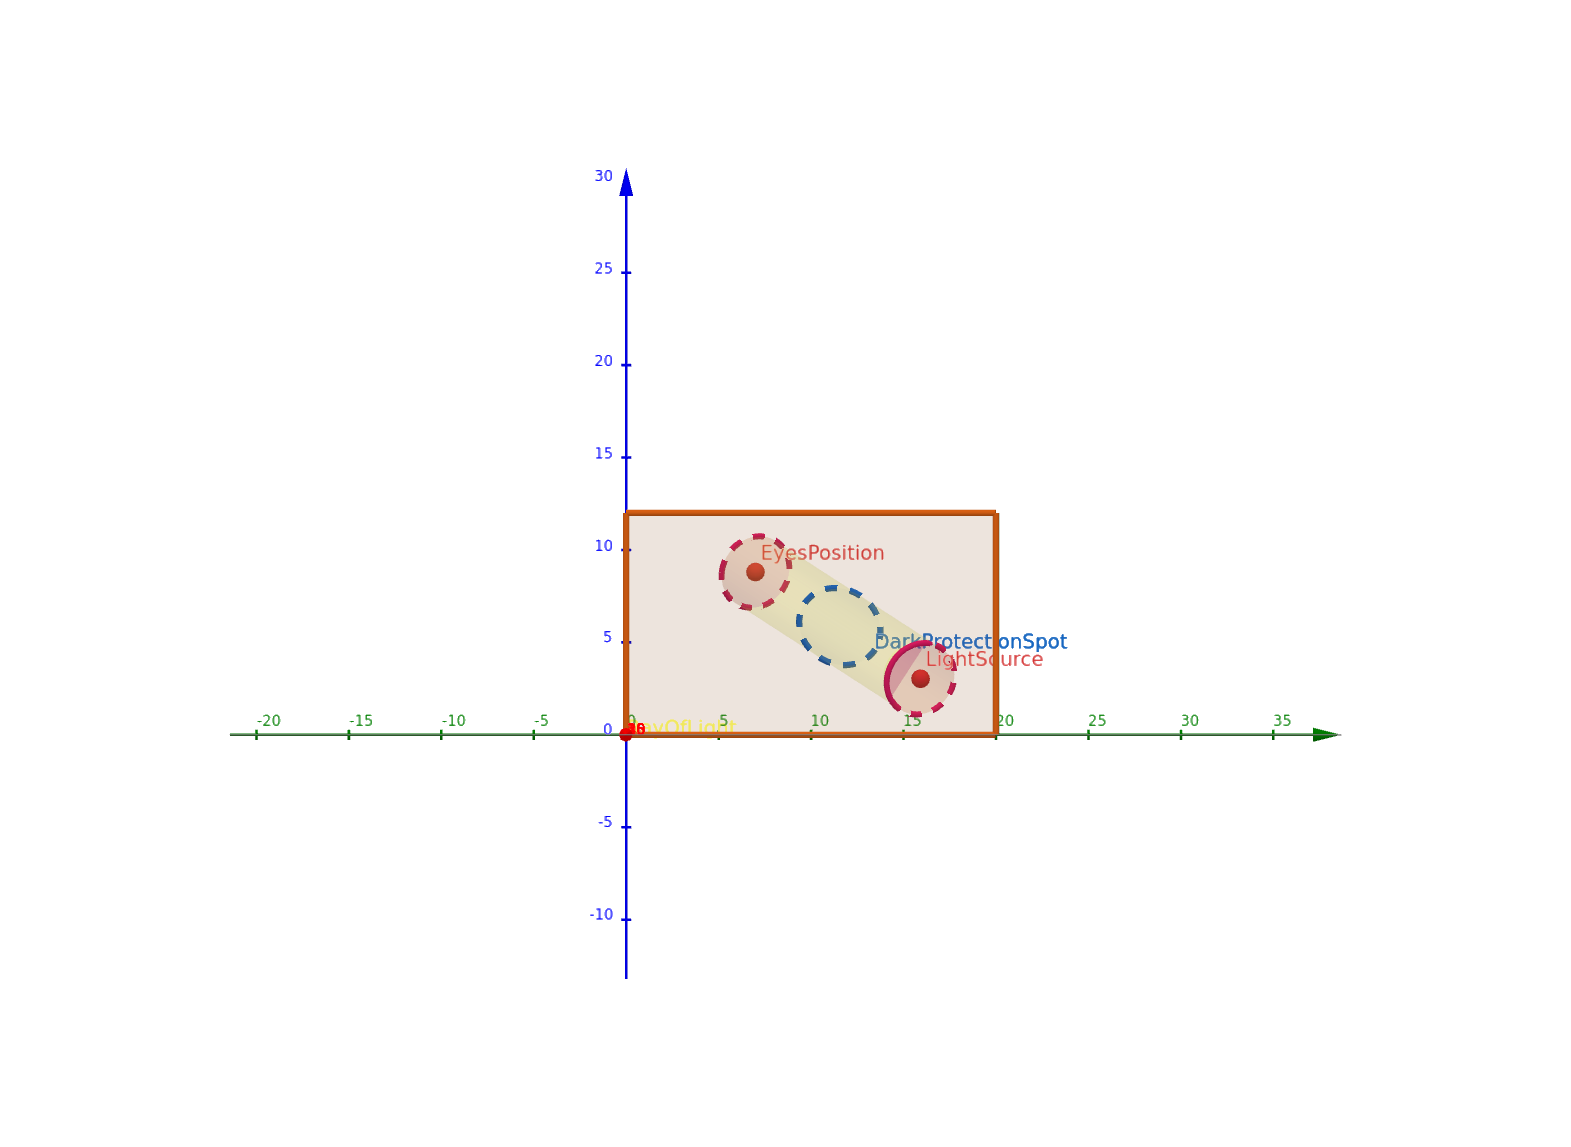
\includegraphics[width=0.8\textwidth]{slike/sustav4}
    \captionsetup{font={small}}
    \caption{Pojednostavljen prikaz sustava u dvodimenzionalnom koordinatnom sustavu [autorski rad]}
    \label{fig:sustav4}
\end{figure}

Nakon razmatranja slike \ref{fig:sustav4} sustava u dvodimenzionalnom polju, dolazi se do zaključka da bi se pozicija pravokutnika crne boje na zaštitnom okviru mogla izračunati pomoću polovišta dužina, što je urađeno programskim kodom \ref{lst:lstlisting_10}.
\pagebreak
\begin{lstlisting}[language=Python, label={lst:lstlisting_10}, firstnumber=33, style=colored, caption={Definicija funkcije $create\_protection\_frame()$}]
def create_protection_frame():
    frame_width = 640
    frame_height = 480

    protection_frame = np.ones((frame_height, frame_width, 3), dtype=np.uint8) * 255

    eye_positions = eyes_position_queue.get()
    light_positions = light_position_queue.get()

    for light_position in light_positions:
        for eye_position in eye_positions:
            eye_x, eye_y, eye_w, eye_h = eye_position
            light_x, light_y, light_w, light_h = light_position

            protection_x = (eye_x + light_x) // 2

            protection_y = (eye_y + light_y) // 2

            cv.rectangle(
                protection_frame,
                (protection_x, protection_y),
                (protection_x + light_w, protection_y + light_h),
                (0, 0, 0),
                -1
            )

    eyes_position_queue.task_done()
    light_position_queue.task_done()

    return protection_frame
\end{lstlisting}

Prikaz funkcioniranja sustava - link na video: \href{https://foi-my.sharepoint.com/:v:/g/personal/spetrovic20_foi_hr/ERfsxYop3VFCnwyEWHfwgokB6hWikBInY5lpKwYVjjt91A?nav=eyJyZWZlcnJhbEluZm8iOnsicmVmZXJyYWxBcHAiOiJPbmVEcml2ZUZvckJ1c2luZXNzIiwicmVmZXJyYWxBcHBQbGF0Zm9ybSI6IldlYiIsInJlZmVycmFsTW9kZSI6InZpZXciLCJyZWZlcnJhbFZpZXciOiJNeUZpbGVzTGlua0RpcmVjdCJ9fQ&e=REgtGV}{https://foi-my.sharepoint.com}

\pagebreak
\chapter{Testiranje sustava}

\pagebreak
\chapter{Zaključak}

Ovdje treba sažeto rezimirati najvažnije rezultate razrade teme rada. Potrebno je sažeto opisati što je predmet rada, koje su metode, tehnike, programski alati ili aplikacije korištene u razradi rada te koje su pretpostavke dokazane, a koje opovrgnute. Sadržajno, ono što se u uvodu rada najavljuje i kasnije je obuhvaćeno u samom radu, moralo bi biti opisano u zaključnom dijelu kroz rezultate rada.

\printbibliography[title=Popis literature]
\addcontentsline{toc}{chapter}{Popis literature}

\listoffigures
\addcontentsline{toc}{chapter}{Popis slika}

\lstlistoflistings
\addcontentsline{toc}{chapter}{Popis programskih kodova}

\end{document}
